\documentclass[
	12pt,				% tamanho da fonte		
	oneside,
	a4paper,			% tamanho do papel.
	chapter=TITLE,
	%sumario=tradicional,
	english,			% idioma adicional
	brazil,				% idioma principal do documento
	]{abntex2}

% ---
% PACOTES
% ---
\usepackage{lmodern}			% Usa a fonte Latin Modern
\usepackage[T1]{fontenc}		% Selecao de codigos de fonte.
\usepackage[utf8]{inputenc}		% Codificacao do documento (conversão automática dos acentos)
\usepackage{indentfirst}		% Indenta o primeiro parágrafo de cada seção.
\usepackage{color}				% Controle das cores
\usepackage{graphicx}			% Inclusão de gráficos
\graphicspath{{figuras/},{figuras/Intro/},{figuras/CAP2/},{figuras/CAP3/},{figuras/CAP4/},{figuras/CAP5/}}
\usepackage{microtype} 			% para melhorias de justificação
\usepackage{booktabs}
\usepackage{float} 				% Set posição da figura
\usepackage[bottom]{footmisc} 
% \usepackage{subfig} 			% Inserir subfiguras
\usepackage[table,xcdraw]{xcolor} 	% Cor de preenchimento das tabelas
\usepackage{multirow} 			%mesclar cel em tabelas
\usepackage{verbatim}			%Inserir codigos fontes e comentários em massa
\usepackage[alf]{lib/abntex2cite}
\usepackage[brazilian,hyperpageref]{backref}
\usepackage{lipsum}				% para geração de dummy text
\usepackage{amsmath}
\usepackage[bottom]{footmisc}
\usepackage{footnote}
%\usepackage{fnpos}
%\usepackage{ftnxtra}
\usepackage{listings} 			%Inserir códigos fontes
\usepackage{rotating} 			%Rotação de páginas
\usepackage{placeins}			% Forçar o posicionamento da figura
\usepackage[top=3cm, bottom=2cm, left=3cm, right=2cm]{geometry} % Margens
\usepackage{algpseudocode,algorithm}
\usepackage{mathrsfs}
\usepackage{hyperref}
\usepackage{caption}
\usepackage{subcaption}
% ---
% Informações de dados para CAPA e FOLHA DE ROSTO
% ---

\titulo{{\normalfont \textbf{CONTROLE EMBARCADO EM ROBÔS COM 
ACIONAMENTO DIFERENCIAL E \emph{ENCODERS} DE BAIXA RESOLUÇÃO.}}}
\autor{LUÍS GABRIEL PEREIRA CONDADOS}
\local{Natal -- RN}
\data{Dezembro de 2020}
\instituicao{
  Universidade Federal do Rio Grande do Norte -- UFRN
  \par
  Departamento de Engenharia de Computação e Automação -- DCA
  \par
  Curso de Engenharia de Computação

}
\tipotrabalho{Relatório técnico}

\preambulo{Trabalho de Conclusão de Curso de Engenharia de Computação da Universidade Federal do Rio Grande do Norte, apresentado como requisito parcial para a obtenção do grau de Bacharel em Engenharia de Computação
\newline 
\newline 
Orientador: Adelardo Adelino Dantas de Medeiros}

% Configurações de aparência do PDF final
% alterando o aspecto da cor azul
\definecolor{blue}{RGB}{41,5,195}
% informações do PDF
\makeatletter
\hypersetup{
     	%pagebackref=true,
		pdftitle={\@title}, 
		pdfauthor={\@author},
    	pdfsubject={\imprimirpreambulo},
	    pdfcreator={LaTeX with abnTeX2},
		pdfkeywords={abnt}{latex}{abntex}{abntex2}{relatório técnico}, 
		colorlinks=true,       		% false: boxed links; true: colored links
    	linkcolor=black,          	% color of internal links
    	citecolor=black,        		% color of links to bibliography
    	filecolor=magenta,      		% color of file links
		urlcolor=blue,
		bookmarksdepth=4
}
\makeatother
% Espaçamentos entre linhas e parágrafos 
\setlength{\parindent}{1.25cm} % Tamanho do parágrafo
\setlength{\parskip}{0.2cm}	% Controle do espaçamento entre um parágrafo e outro

%\onelineskip % Controle do espaçamento entre um parágrafo e outro

\makeindex % compila o indice

% Início do documento
% ----
\begin{document}

% Seleciona o idioma do documento (conforme pacotes do babel)
%\selectlanguage{english}
\selectlanguage{brazil}

% Retira espaço extra obsoleto entre as frases.
\frenchspacing 

% ----------------------------------------------------------
% ELEMENTOS PRÉ-TEXTUAIS
% ----------------------------------------------------------
\pretextual

% Capa
\imprimircapa

% Folha de rosto
\imprimirfolhaderosto

% Inserir folha de aprovação
\begin{folhadeaprovacao}
	
	\begin{center}
		{\ABNTEXchapterfont\large\imprimirautor}
		
		\vspace*{\fill}\vspace*{\fill}
		\begin{center}
			\ABNTEXchapterfont\bfseries\Large\imprimirtitulo
		\end{center}
		\vspace*{\fill}
		
		\hspace{.45\textwidth}
		\begin{minipage}{.5\textwidth}
			\imprimirpreambulo
		\end{minipage}%
		\vspace*{\fill}
	\end{center}
	
% 	Trabalho aprovado. \imprimirlocal, 14 de Dezembro de 2020:
    \textbf{Trabalho  de  Conclusão  de  Curso  apresentado  à  banca  examinadora  composta  pelos  seguintes  membros:}  
	
	\setlength{\ABNTEXsignwidth}{14cm}
	\assinatura{\textbf{Prof. Dr. Adelardo Adelino Dantas de Medeiros - Orientador} \\ DCA/UFRN} 
	\assinatura{\textbf{Prof. Dr. Carlos Eduardo Trabuco Dórea} \\ DCA/UFRN}
	\assinatura{\textbf{Prof. Dr. Pablo Javier Alsina} \\DCA/UFRN}
	
	\begin{center}
		\vspace*{0.5cm}
		{\large\imprimirlocal}
		\par
		{\large\imprimirdata}
		\vspace*{1cm}
	\end{center}
	
\end{folhadeaprovacao}

% Dedicatória
\begin{dedicatoria}
	\vspace*{\fill}
	\centering
	\noindent
	\textit{Escreva aqui sua dedicatória}
	 \vspace*{\fill}
\end{dedicatoria}

% Agradecimentos
\begin{agradecimentos}

Agraço primeiramente à Deus, que me abençoou com a família que tenho, que sem o suporte e confiança incondicionais, esse trabalho não seria possível. Em especial agradeço a minha avó, \textbf{Maria Eliza}, pelo incentivo, suporte e pela ótima criação. Sem dúvidas esse trabalho não seria possível sem o apoio dela.

Ao meu orientador e orientador da Equipe POTI Professor Dr. Adelardo Adelino, pelos ensinamentos e por me apresentar a Equipe, que fez com que eu despertasse um grande interesse pela área da robótica, bem como foi de grande valor para o meu aprimoramento durante o curso.

Agradeço aos atuais integrantes da equipe POTI \textbf{Daniel Morais} e \textbf{Victor Duarte} pelo companheirismo e ajuda na elaboração deste trabalho.

Obrigado também a todos os professores e colegas do curso de Engenharia de Computação que fizeram ou fazem parte da minha vida acadêmica, pelas ajudas e ensinamentos durante todo o curso.

Por fim, aos que direta ou indiretamente me ajudaram de alguma forma, mas não foram mencionados aqui.
\end{agradecimentos}

% ---
% Epígrafe
% ---
\begin{epigrafe}
	\vspace*{\fill}
	\begin{flushright}
		\textit{``Feliz o homem que encontrou a sabedoria e alcançou o entendimento,\\
			porque a sabedoria vale mais do que a prata, \\
			e dá mais lucro que o ouro."\\
			(Bíblia Sagrada, Provérbios 3, 13-14)}
	\end{flushright}
\end{epigrafe}

% RESUMO
% resumo na língua vernácula (obrigatório)
\setlength{\absparsep}{18pt} % ajusta o espaçamento dos parágrafos do resumo
\begin{resumo}

Este trabalho apresenta uma proposta e testa na prática um sistema de observação e controle de velocidade para motores de corrente contínua equipados com \emph{Encoders} de baixa resolução. O trabalho tem como aplicação alvo mini robôs de acionamento diferencial. O sistema proposto foi implementado no microcontrolador (\emph{ESP32}) e mostrou-se, pelos resultados experimentais, ser capaz de controlar a velocidade do par motor-roda de robôs com acionamento diferencial (com \emph{Encoders} rotativos de baixa precisão) de forma a conseguir reduzir as assimetrias desses. Fez-se uso de um esquema de controle com dois graus de liberdade, do tipo \emph{Feedforward}/\emph{Backward} e usou-se o filtro de \emph{Kalman} para realizar a estimativa da velocidade, com o objetivo de reduzir o erro de quantização dos sensores.

% Escreva seu resumo aqui. Ele deve ser parágrafo único e sem récuo na primeira linha.
%  \lipsum[1-1]
 
%  \noindent
 \textbf{Palavras-chaves}: Controle Embarcado. Motores CC. Filtro de \emph{Kalman}. \emph{ESP32}. Robôs com acionamento diferencial.
\end{resumo}
% ---
% resumo em inglês
\begin{resumo}[Abstract]
	\begin{otherlanguage*}{english}
	
		This work presents a proposal and tests in practice a speed observer and controller for DC motors equipped with low-resolution Encoders. This work's target application was mini differential drive robots. The system was implemented in the microcontroller (ESP32) and shown, by experimental results, to be able to control the speed of the motor-wheel pairs of differential drive robots (with low-precision rotary encoders) way to reduce the asymmetries of them. A control scheme with two degrees of freedom, of the type Feedforward / Backward, was used, with the Kalman filter as the speed estimator, with the objective of reducing the sensors quantization error.
	
	\vspace{\onelineskip}
	\noindent 
	\textbf{Keywords}: Embedded Control. DC Motors. Kalman Filter. ESP32. Robots with differential Drive.
	\end{otherlanguage*}
\end{resumo}

% ---
% inserir lista de ilustrações
\pdfbookmark[0]{\listfigurename}{lof}
\listoffigures*
\cleardoublepage

% inserir lista de tabelas
\pdfbookmark[0]{\listtablename}{lot}
\listoftables*
\cleardoublepage

% inserir lista de abreviaturas e siglas
\begin{siglas}
% \item[HTML] \textit{HyperText Markup Language}
% \item[JSON] \textit{JavaScript Object Notation}
% \item[REST] \textit{Representational State Transfer}
% \item [] \textit{}
\item [$\mu{}C$] \textit{Microcontrolador}
\item [GPIO] \textit{General Purpose Input/Output}
\item [SDK] \textit{Software Development Kit}
\item [RTOS] \textit{Real Time Operating System}
\item [NPR] \textit{Número de Pulsos por Revolução}
\item [PPR] \textit{Pulsos Por Revolução}
\end{siglas}

% inserir lista de símbolos
% \begin{simbolos}
%   \item[$ \Gamma $] Letra grega Gama
%   \item[$ \Lambda $] Lambda
%   \item[$ \zeta $] Letra grega minúscula zeta
%   \item[$ \in $] Pertence
% \end{simbolos}

% inserir o sumario
\pdfbookmark[0]{\contentsname}{toc}
\tableofcontents*
\cleardoublepage

\textual

% Capitulo 1: Introdução
\chapter[Introdução]{Introdução}
\label{ch:introdução}
% [High-Performance Speed Control of Electric Machine Using Low-Precision Shaft Encoder]

% SPEED CONTROL through accurate speed detection is
% an essential requirement in the field of high-performance
% motion control like machine tool applications. An ordinary
% speed control uses average speed information as a speed
% feedback signal that is obtained by counting the increased
% number of encoder pulses during the detection time or the
% sampling interval [1]. However, the average speed information
% is not good enough to control the motor speed precisely
% because average detection lag is produced and the speed
% information is lost during the sampling interval, especially in
% a low-speed range when a low-precision shaft encoder is used.
% Therefore, instantaneous speed observers based on distur-
% bance torque observer have been reported as a better method
% to avoid unstable system which can be caused by making
% sampling time longer to obtain more encoder pulses [2]–[4].
% However, the observers do not have good noise-rejection prop-
% erties in noisy environment in comparison with the Kalman
% filter known as an optimal state estimator [5]. The Kalman
% filter is a stochastic estimator that possesses the smoothing
% properties and the noise-rejection capability robust to the
% process and measurement noise. Even though the Kalman filter


% [Low Speed Control of Permanent Magnet Synchronous Motor Based on Instantaneous Speed Estimation]

% Abstract - Incremental-type encoder is widely used for speed
% detection in servo system. However, the speed controller of the
% system usually becomes unstable at low speed range using
% average speed estimation method. An instantaneous speed
% estimation scheme for low speed control of permanent magnet
% synchronous motor is proposed. The speed estimation adopts a
% full order state observer to calculate feedback speed. The method
% can achieve good response because it is possible to detect the
% speed exactly without detection dead time. The observer design
% considerations for application are analyzed. Furthermore, inertia
% identification based on recursive extended least square algorithm
% is presented to reduce sensitivity of the speed estimation.
% Experimental results show that low speed control performance
% using the instantaneous speed estimation with inertia
% identification is superior to that of conventional one.

% [...]

% Presently, incremental-type encoder is the most
% typical speed and position sensor for servo system considering
% the cost and the performance. Speed detection using the
% encoder is calculated by counting the number of pulses
% generated by the encoder and interval between them [1], [2].
% This method detects the averaging speed, and therefore, it
% causes a detection dead time. Under low speed conditions,
% especially, where the interval between the pulses is wider than
% a speed control period, the detection dead time usually makes
% the speed controller unstable.

% To improve the performance of the speed control system
% which has been degraded by the detection dead time, several
% instantaneous speed observers have been proposed by using
% state observation theory. Instantaneous speed estimation using
% reduced-order disturbance torque observer has simple
% structure and easy to implement [3], [4]. But the gains of
% observer and controller are limited to increase in real
% application for mechanical noise and oscillation of system.
% Recently, a full order state estimation algorithm has been
% proposed which is based on the optimal state estimation theory
% like Kalman filter [5], [6]. But this scheme is complicated to
% implement since it needs large calculation.


% [Speed Measumment Using Rotary Encoders for High Performance ac Drive]
% Abstd - Most of high performance speed control of electrical
% motors, like ac Vector Conhol, use mtay encoders. The accuracy
% obtaining the mtor speed fmm encoder signals is an essential
% mquimment to achieve a good dynamic msponse, but it usually
% implies a delay in the speed conbol loop, which can cause stability
% problems.

% Ótimo Exemplo de "Trabalhos relacionados"
% A plenty of groundwork has been done for this
% paper and every important point that is to be
% highlighted is considered from previous literature.
% The book 'The 8051 Microcontroller and
% Embedded Systems Using Assembly and C, 2nd
% edition Mohammad Ali Mazidi, Janice Gillispie
% Mazidi, Rolin D. McKinlay presented the
% programming of microcontroller 8051 for the
% generation of pulses[I].The book 'Electrical
% Machines', P.S. Bimbra, Khanna Publishers
% presented the working principle of dc motor. And
% the methods of speed control of dc motor are
% explained [2].The book 'Fundamentals of Electric
% Drives', Gopal K. Dubey explained the pulse width
% modulation technique and the speed control of dc
% motor using pulse width modulation is explained.
% The effective output voltage can be varied by
% varying the duty cycle of the pulse [3].The book
% Micro Controller Architecture,
% 'The 8051
% Programming and Applications', Kenneth J.Ayala
% presented the ADC interfacing and LCD interfacing
% with the micro controller 8051 [4].

Em robótica móvel (mas não limitando-se) é comum o uso de controladores que possuem como saída as velocidades de giro que devem ser atingidas pelos conjuntos motor-roda do robô. Como por exemplo: controladores estabilizantes, seguidores de caminho e seguidores de trajetória. Portanto é essencial garantir que os motores tentem/consigam atingir essas velocidades, preferivelmente por meio do uso de controladores embarcados no robô. Com isso vem a necessidade do sensoriamento (\emph{Feedback}) e do processamento extra por parte do sistema embarcado do robô. O que pode se um problema em aplicações com baixo poder computacional e/ou restrições com relação ao uso de sensores de alta precisão. Sejam essas limitações econômicas ou estruturais.\\

\section{Contextualizando}
% Main ref for this first sentence.  % [A Simple Speed Feedback System for Low Speed DC Motor Control in Robotic Applications] como ref. para o começo da intro.
Uma forma muito comum de acionamento de motores de corrente continua (CC) é por meio da modulação por largura de pulso, ou do inglês Pulse Width Modulation (PWM), que consiste basicamente em manipular a tensão média de alimentação do motor por meio de sinais digitais. É comum em certas aplicações o uso do sinal \emph{PWM} para manipular a velocidade do motor, ou seja, um controle de malha aberta, esse tipo de sistema apenas regula o quão rápido o motor irá girar. Porém na maioria das aplicações o controle em malha aberta não é suficiente, como por exemplo, não há garantias que se aplicado tensões iguais (\emph{PWM}) em ambos os motores de um robô com acionamento diferencial (robôs com duas rodas tracionadas e independentes) o movimento será estritamente linear \cite{simple_speed_feedback}, isso devi-se as diferenças entre os dois conjuntos de motores/rodas que fazem com que esses não girem a uma mesma velocidade, mesmo sobre uma mesma tensão.\\

Em contraste com o sistema de malha aberta, um sistema de malha fechada utiliza o sinal da saída da planta como \emph{Feedback} para realizar o controle. Esse tipo tende a manter a variável que se está controlando o mais próximo possível da referência desejada. Isso é feito usando a diferença entre a saída e a entrada (erro) como meio de controle. \\ %ta ruim essa explicação!

% [Speed Measurement Algorithms for Low-Resolution Incremental Encoder Equipped Drives: a Comparative Analysis]
Portando, ter-se um bom \emph{Feedback} em sistemas de controle em malha fechada é de extrema importância \cite{analise_incr_enc}, \cite{simple_speed_feedback}, tanto para se trabalhar em alta performance, quanto para garantir a estabilidade do sistema. No contexto de controle de rotação de motores, os sensores mais comuns são os codificadores de eixo (\emph{Encoders}). Os dois principais tipos são: \emph{Encoders} absolutos e os incrementais. O primeiro fornece a informação da posição angular absoluta e o segundo uma informação da variação de giro. \\

A resolução desses sensores influencia fortemente no desempenho e até mesmo na viabilidade do controlador, porém, sensores com resoluções maiores são, por consequência, mais caros, fazendo-se que seja necessário um \emph{Trade-off} \cite{analise_incr_enc}, \cite{low_precision_encoder01} entre custo e desempenho. Existem diversas técnicas que tentam melhorar a estimativa da velocidade sem que seja necessário o uso de sensores mais precisos, um tipo de técnica que geralmente é usada para esse fim são os estimadores/observadores de estado \cite{analise_incr_enc}, \cite{speed_observer_IA}, \cite{observer_speed}, que calculam uma estimativa da velocidade a partir dos dados do sensor e/ou de algum conhecimento sobre o comportamento do sistema. Porém, também há um \emph{Trade-off} com relação a qual estimador usar. Bons estimadores exigem mais poder computacional e/ou exigem que tenha-se mais conhecimento sobre a planta. O que pode ser um problema para certos tipos de aplicações, como é o caso de uma aplicação que deve rodar em um microcontrolador ($\mu$C) de um robô.\\

\section{Trabalhos Relacionados}
% \section{Estado da Arte}

O controle (embarcado ou não) de velocidade de motores e o estudo sobre observadores de estados voltados para estimação dessa velocidade, usando-se na maioria dos casos, \emph{Encoders} incrementais são assuntos bastante estudados, tanto individualmente quanto separadamente. No trabalho \cite{low_precision_encoder01} por exemplo, os autores demostram em por seus resultados uma melhora no desempenho do controle de velocidade do motor usando-se uma técnica de mínimos quadrados recursivos (\emph{recursive least squares}) para fazer o ajuste automático (\emph{Self-tunning}) dos parâmetros do controlador e os parâmetros do observador de velocidade por filtro de \emph{Kalman}. 

Em \cite{Y_HORI_01} e \cite{Y_HORI_02} o autor ...


Diante do exposto, é notável que diferentes estratégias estão sendo implementadas com o mesmo intuito: ...

\section{Motivações e Objetivos}
% V2
% MOTIVAÇÃO!!!
Existem diversos desafios no projeto de robôs pequenos, além da questão mecânica, o tamanho reduzido também restringe a possibilidade de se usar \emph{Hardwares} com mais capacidade computacional, além dos tipos e a quantidade de sensores que podem ser usados. Robôs como os da equipe Poti de Futebol de robôs (do Departamento de Computação e Automação (DCA) da UFRN), que são voltados para a participação na \emph{Latin American Robotic Competition} (LARC) na categoria \emph{IEEE Very Small Size Soccer} (VSSS), têm dificuldades para conseguirem comportar um \emph{Hardware} capaz de executar um controle digital de velocidade para ambos os motores, além de possuírem sensores com uma baixa acurácia, dificultando assim o bom desempenho do sistema de controle.\\

O objetivo geral deste trabalho é projetar um sistema que realize o controle de velocidade dos motores de um robô com acionamento diferencial e que utiliza um estimador de velocidade ótimo sobre medições feitas com \emph{Encoders} de baixa resolução. Para a validação do trabalho foi feito a implementação do sistema proposto, testado em robôs reais e feito análises da eficiência dos controladores com relação a diminuição das assimetrias dos conjuntos motor-roda, bem como a qualidade da filtragem/estimativa da velocidade. %Os robôs utilizados foram desenvolvidos como parte do trabalho, por isso o detalhe de seu projeto também foi explorado.

% ****************************************************
% Intro à Robocup, IEEE VSSS e Equipe Poti
\section{Equipe Poti de Futebol de Robôs}
\label{sec:Equipe_Poti}

A Equipe Poti de Futebol de Robôs surgiu no Departamento de Engenharia de Computação e Automação da Universidade Federal do Rio Grande do Norte (DCA-UFRN), sendo participante na categoria \emph{IEEE Very Small Size Soccer}.\\

Nessa categoria duas equipes de 3 robôs de até 7,5 x 7,5 x 7,5cm jogam uma partida de futebol. Os robôs são controlados remotamente por um computador, mas sem intervenção humana \cite{VSSS}. O computador processa a imagem de uma câmera de vídeo colocada acima do campo e comanda os robôs. Na equipe Poti cada robô possui uma função no jogo, como: o goleiro, o atacante e o defensor, de forma que dependendo da estratégia de jogo eles podem se alternarem para melhor desempenho do time. A arquitetura do sistema do Futebol de Robôs do Time Poti é formada por vários módulos, sendo eles: visão, localização, estratégia, controle e transmissão.\\

O módulo de visão consiste de uma câmera que fotografa o campo com os jogadores e a bola, a taxa de captura da câmera é o fator que limita o tempo de amostragem de todo o sistema, atualmente a equipe utiliza uma taxa de amostragem de $100$ quadros/\emph{Frames} por segundo(FPS). O módulo de localização fornece a posição da bola e dos jogadores através das cores que foram predefinidas. O módulo de estratégia é responsável pelo próximo passe que os robôs deverão executar, a partir das imagens atuais. O módulo de controle é responsável por converte as referências de posição e orientação, definidas pela estratégia, em sinais que correspondem as velocidades que devem ser aplicadas nas rodas direita e esquerda de cada robô e o módulo de transmissão envia esse sinal para os robôs \cite{POTI}.\\

% O \textit{Hardware} projetado para esses robôs conta com um microcontrolador dual core de 32\emph{bits} da empresa \emph{Espressif Systems} (ESP32) e \textit{Encoders} magnéticos de $3$ pulsos por revolução por canal. Foi embarcado  nesse microcontrolador um controle de velocidade angular do tipo  \textit{FeedForward}/\textit{Backward}(PID), que deve atuar no par de motores dos robôs de  forma a controlar suas velocidades bem como reduzir as assimetrias entre  os motores direito e esquerdo.\\

% Usando a interface \textit{Bluetooth} presente no microcontrolador, foi criado um  protocolo simples de comunicação para realizar operações de telemetria e telecomando nos robôs. O \textit{Firmware} opera utilizando os dois núcleos  executando tarefas distintas: um núcleo é responsável pela comunicação  com o servidor, por meio do \textit{Bluetooth} e do protocolo criado, bem como  por tratar as interrupções geradas pelos \textit{Encoders} rotativos magnéticos;  já o outro núcleo executa a rotina de controle, com um período de amostragem de pelo menos $5$ms, para operar em uma frequência de pelo menos duas vezes mais rápido que o sistema que está rodando no \emph{Host}, que como já mencionado trabalha até à $100$Fps ($10$ms).\\

% Para medir a velocidade de rotação, foram utilizados \textit{Encoders} magnéticos  rotativos, com resolução de $3$ pulsos por canal por revolução do eixo do motor. Para diminuir a  incerteza na estimativa da velocidade, é aplicado um filtro de \textit{Kalman},  considerando a planta (motores) como um sistema de primeira ordem. Os  parâmetros da planta (constante de tempo, zona morta e ganho \emph{PWM} x  Velocidade angular) são estimados/calculados por mínimos quadrados na  rotina de calibração presente no \textit{Firmware}, sendo em seguida utilizados  para determinar os parâmetros do controlador.

\section{Estrutura do Trabalho}

Este trabalho apresenta uma introdução sobre o tema, mostrando os fatores que motivam a implantação da ideia, além da justificativa e dos objetivos. Em sequência, o \autoref{ch:referencial_teorico} aborda os principais conceitos teóricos e técnicos utilizados no trabalho. O \autoref{ch:metodologia}, por sua vez, descreve os detalhes de organização e implementação de todas as partes do sistema proposto, bem como os procedimentos adotados para os testes e validação, enquanto o \autoref{ch:resultados} trata de mostrar os resultados obtidos experimentalmente. O \autoref{ch:Discussão} apresenta discussões sobre os resultados apresentados no capitulo anterior, frisando os principais pontos. Por fim, o \autoref{ch:conclusao} traz as principais conclusões e contribuições deste trabalho, bem como sugestões de trabalhos futuros.

% Organização do trabalho
% Este trabalhado é organizado da seguinte maneira: O Capítulo 1 corresponde à introdução do trabalho, por meio da qual é feita uma contextualização do problema e a proposta de solução para o mesmo; o capítulo 2 traz a fundamentação teórica utilizada para o desenvolvimento deste trabalho; no capítulo 3, os objetivos gerais e específicos são abordados; no capítulo 4 são apresentados os materiais e métodos utilizados para implementação do sistema; o capítulo 5 contém os resultados e discussões em que podem ser observadas as telas do sistema proposto; no capítulo 6 as conclusões deste trabalho são levadas em consideração, assim como sugestões de trabalhos futuros.

% Revisão bibliográfica / Referencial teórico
\chapter[Referencial Teórico]{Referencial Teórico}
\label{ch:referencial_teorico}

Nesta seção serão apresentados os principais conceitos utilizados neste trabalho, sendo eles: motores de corrente contínua; Filtro de \emph{Kalman}; Método dos mínimos quadrados; Introduz alguns conceitos chaves sobre a teoria de controle; Breve explicação sobre a comunicação \emph{Bluetooth}; Detalhes sobre o funcionamento dos \emph{Encoders} rotativos incrementais e por fim fala sobre o funcionamento básico dos sinais PWM.
%********************************************************************
\section{Motor de Corrente Contínua}
\label{sec:motor_ref_teo}
% Introduzir o que funcionamento básico de um motor CC
% deixar claro qual o tipo será apresentado/utilizado no trabalho (motor CC de campo magnético fixo e com "escova")
Como o próprio nome indica, os motores CC são acionados por uma fonte de corrente contínua. São motores que possuem ímãs permanentes ou então têm campo e armadura. Esse tipo de motor é amplamente utilizado em diversas aplicações.

Ele é constituído basicamente pelo enrolamento de armadura, enrolamento de campo, comutador e as escovas, onde:

\begin{itemize}
    \item Enrolamento de armadura: é localizado na parte giratória do motor de CC (rotor) que é responsável por produzir o torque que o movimenta, bem como a tensão de saída quando em modo de gerador.
    
    \item Enrolamento de campo: parte fixa responsável pelo fluxo magnético constante que irá atravessar a armadura. 
    
    \item Comutador: Possui a função de manter a corrente da armadura circulando no mesmo sentido, fazendo com que o torque mantenha seu sentido para uma tensão de entrada constante.
    
    \item Escovas: é por onde acontece o contato do enrolamento de armadura com a fonte de alimentação.
\end{itemize}


As máquinas de corrente contínua são bastante utilizadas em sistema de controle em razão do seu comportamento essencialmente linear [apostilha:modelagem]. O diagrama esquemático de uma máquina (motor ou gerador) CC é mostrado na figura \ref{fig:modelo_motor_dc}. O enrolamento de campo tem resistência $R_f$ e indutância $L_f$ e o enrolamento de armadura tem resistência $R_a$ e indutância $L_a$. As correntes e tensões nos enrolamentos de campo e de armadura $i_f$, $v_f$, $i_a$ e $v_a$, respectivamente. A tensão induzida na armadura é $v_g$. O torque e a velocidade angular no eixo do rotor são $\tau$ e $\omega$, respectivamente.

A tensão induzida no enrolamento de armadura é dada por:

\begin{equation}
    v_g = K_{1}\phi\omega
\end{equation}

E o torque é dado por:

\begin{equation}
    \tau = K_{1} \phi i_a 
\end{equation}

Onde $K_1$ é um parâmetro determinado pela estrutura física da máquina e $\phi$ é o fluxo magnético. Supondo que a máquina esteja operando na zona linear (ou seja, que o núcleo não esteja saturado), o fluxo é dado pela equação:

\begin{equation}
    \phi = K_{2}i_f
\end{equation}

Onde $K_2$ é uma constante e depende das características magnéticas do núcleo e do enrolamento de campo.

Motores geram potência mecânica, de forma que a velocidade de rotação $\omega$ é o sinal de saída e a tensão $v_a$ aplicada é o sinal de entrada. 

\begin{figure}[H]
    \centering
    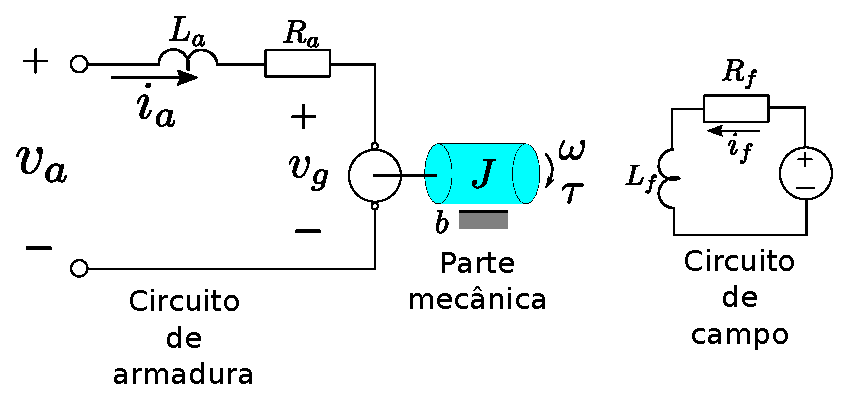
\includegraphics[width=0.5\textwidth]{figuras/ilustracoes/esquematico_motor_dc.eps}
    \caption{Diagrama esquemático de um motor CC.}
    \label{fig:modelo_motor_dc}
\end{figure}


A figura \ref{fig:modelo_motor_dc} apresenta o diagrama esquemático para um motor de corrente contínua (CC) controlado pela armadura, ou seja, o sinal de entrada é a tensão aplicada na armadura ($v_a$). Nesse diagrama a carga está sendo modelada por um momento de inércia $J$ e um atrito viscoso de coeficiente $b$.

\begin{align*}
    v_g &= K_{1}\phi\omega= K_{1}K_{2}i_{f}\omega = K_{m}\omega\\
    \tau &= K_{1} \phi i_{a}= K_{1} K_{2}i_{f} i_{a} = K_{m}i_{a}
\end{align*}

A constante $K_{m}$ é conhecida como a constante do motor. Devido a relação apresentada anterior é possível modelar o circuito equivalente do motor CC como na imagem \ref{fig:eq_eletrico_motorcc}.
% figura retirada do livro texto da disciplina de modelagem.
\begin{figure}[H]
    \centering
    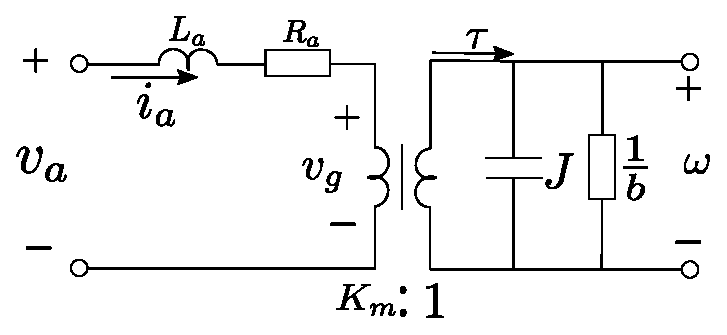
\includegraphics[width=0.6\textwidth]{figuras/ilustracoes/circuito_equivalente_motor_cc.eps}
    \caption{Equivalente elétrico de um motor CC}
    \label{fig:eq_eletrico_motorcc}
\end{figure}

Do circuito da figura \ref{fig:eq_eletrico_motorcc} extrai-se a seguinte função de transferência:

\begin{equation*}
    \frac{\Omega(s)}{V_a(s)} = \frac{K_m}{JL_{a}s^2 + \left(JR_a + BL_a \right)s + BR_a + K_{m}^2} \left[\frac{ rad.s^{-1}}{V}  \right]
\end{equation*}

Caso a impedância da armadura seja desprezada $(L_a \xrightarrow{} 0)$:

\begin{equation}
    \frac{\Omega(s)}{V_{a}(s)} = \frac{K_m}{JR_{a}s + BR_{a} + K_{m}^2} = \frac{K}{T_{m}s + 1} \left[\frac{ rad.s^{-1}}{V}  \right]
    \label{eq:motor_transf_func}
\end{equation}

Portando, caso a impedância da armadura seja desprezada, a função de transferência do motor que relacionada a velocidade angular com a tensão de entrada se comporta como um sistema de primeira ordem. A maior dificuldade encontrada ao se controlar motores CC é a amplitude elevada da corrente de armadura, o que requer a utilização de sinal $v_a$ de entrada fornecido por uma fonte de alta potência [apostilha].
\input{textuais/referenciais_teoricos/sistemas_de_primeira_ordem}
\section{Sistemas de Controle}

O controle automático é um componente importante e intrínseco em sistemas de veículos espaciais, sistemas robóticos, modernos sistemas de manufatura e quaisquer operações industriais que envolvam o controle de temperatura, pressão, umidade, viscosidade, vazão etc \cite{ogata2011engenharia} [Okata:Eng.Controle Moderno]. Um problema de controle consiste em determinar uma forma de afetar um dado sistema físico de modo que seu comportamento atenda às especificações de desempenho previamente estabelecidas. Como, normalmente, não é possível alterar a estrutura funcional do sistema físico em questão, a satisfação das especificações de desempenho é atingida mediante o projeto e implementação de controladores (compensadores) [apostilha]. Algumas \textbf{definições/terminologias} comuns no contexto de sistema de controle são apresentadas a seguir.

%[Okata:Eng.Controle Moderno]
Segundo \cite{ogata2011engenharia}.
\textbf{Sinal de controle ou variável manipulada.} Como o próprio nome indica, é a grandeza controlada/manipulada. É o sinal que é modificado pelo controlador, de modo a afetar a variável que se está controlando. Geralmente o sinal de controle é a saída do sistema (entrada da planta).\\

\textbf{Planta.} Uma planta pode ser um equipamento, parte de um equipamento ou um conjunto que funciona de maneira integrada, com o objetivo de realizar uma determinada tarefa. Pode ser qualquer mecanismo/objetivo físico a ser controlado (como por exemplo, um motor, um reator ou qualquer componente mecânico no geral).

\textbf{Processos.} Caracteriza-se por ser qualquer operação com um desenvolvimento por mudanças graduais e progressivas que se sucedem de forma a conduzir um resultado ou uma determinada finalidade.

\textbf{Sistemas.} É uma combinação de vários componentes que trabalham em conjunto para atingir um determinado objetivo. O conceito pode ser aplicado tanto para fenômenos físicos quanto para fenômenos abstratos.

\textbf{Distúrbios.} É uma interferência (sinal adverso) que influência na saída de um sistema. Pode ocorrer internamente ao sistema quando externamente.


\textbf{Controle.} Ação por meio da qual se manipula um sistema físico visando fazer com que este atenda um determinado conjunto de especificações determinadas a priori.

\textbf{Controlador.} Dispositivo utilizado para realizar o controle de um sistema físico.



\textbf{Sistema de controle em malha aberta (\emph{Feedforward}).} Sistema de controle que não possui a entrada influenciada pela saída do sistema. Isso quer dizer que, o sinal de saída não é medido nem realimentado para comparação com a entrada (Ver Figura \ref{fig:ilustracao_sistema_malha_aberta}). Devido a natureza desse tipo de controle, a entrada de referência é mapeada para uma saída fixa do controlador. Dessa maneira, a precisão do sistema depende de uma calibração para melhor ajustar/mapear a referência em um determinado sinal de controle.

\begin{figure}[H]
    \centering
    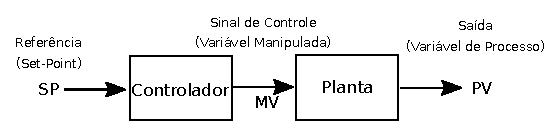
\includegraphics[width=0.8\textwidth]{figuras/ilustracoes/diagrama_sistema_malha_aberta.eps}
    \caption{Diagrama de exemplificação de sistema de controle em malha aberta.}
    \label{fig:ilustracao_sistema_malha_aberta}
\end{figure}

\textbf{Sistema de controle em malha fechada.} Difere essencialmente do em malha aberta, pois neste tipo a entrada do controlador é influenciada pela saída da planta (variável de processo) (Ver Figura \ref{fig:ilustracao_sistema_malha_fechada}). Esse tipo de sistema de controle também é denominado de controle com realimentação (controle com \emph{Feedback}). A relação entre a saída e a entrada de referência se dar por meio da comparação entre elas, utilizando a diferença como meio de controle.

\begin{figure}[H]
    \centering
    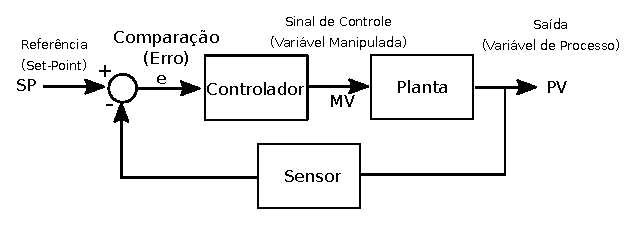
\includegraphics[width=0.8\textwidth]{figuras/ilustracoes/diagrama_sistema_malha_fechada.eps}
    \caption{Diagrama de exemplificação de sistema de controle em malha fechada.}
    \label{fig:ilustracao_sistema_malha_fechada}
\end{figure}


Segundo [Okata] as principais vantagens do sistema de controle em malha aberta são:
\begin{enumerate}
    \item São de fácil construção/implementação e fácil manutenção.
    \item Não apresentam problemas de estabilidade.
    \item São mais adequados em situações em que a medição precisa da saída é um problema.
\end{enumerate}

E algumas desvantagens:

\begin{enumerate}
    \item Distúrbios e mudanças na calibração causam erros, e a saída pode apresentar diferenças
    em relação ao padrão desejado.
    \item Para que a saída mantenha a qualidade requerida, é necessária uma regulagem periódica.
\end{enumerate}


\subsection{Controlador PID}
% Controlador PID
% Controlador malha aberta Feedforward
Um controlador clássico do tipo \emph{Feedback} e que ainda é muito utilizado é o controlador proporcional Integral derivativo (PID). Como o próprio nome indica, esse tipo de controlador une as ações derivativa, integral e proporcional. A ação proporcional faz com que o erro diminua e influência no tempo de resposta do sistema, a ação integral elimina o erro de regime e a ação derivativa influência no tempo de resposta do sistema, por meio da antecipação do erro.

Definindo-se os seguintes sinais no tempo: $u(t)$ como sinal de saída (sinal de controle) e $e(t)$ como o erro entre a referência e o valor atual da saída da planta, o controlador pode ser definido como:

\begin{equation}
    u(t) = K_{p}e(t) + K_{i} \int^{t}_{0}e(\tau)d\tau + K_{d}\frac{d e(t)}{dt}
\end{equation}

Aplicando a transformada \emph{Laplace} temos,

\begin{equation}
    \frac{U(s)}{E(s)} = K_{p} + \frac{K_{i}}{s} + K_{d}s
\end{equation}

Sendo,

\begin{itemize}
    \item $K_p$: O ganho proporcional.
    \item $K_i$: Ganho integral.
    \item $K_d$: Ganho derivativo.
    \item $s$: Frequência complexa.
\end{itemize}

Esse tipo de controlador pode ser utilizado em mais três formas básicas além do padrão PID: Controle Proporcional (P). Apenas a ação proporcional; Controle Proporcional Integral (PI) e Controle Proporcional Derivativo (PD).

\begin{figure}[H]
    \centering
    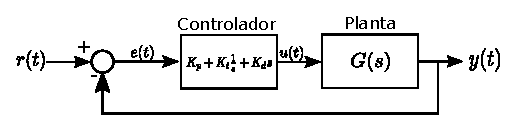
\includegraphics[width=\textwidth]{figuras/ilustracoes/diagrama_controlador_PID.eps}
    \caption{Diagrama de um sistema controlado por PID.}
    \label{fig:diagrama_controlador_PID}
\end{figure}

A Figura \ref{fig:diagrama_controlador_PID} ilustra em diagrama de blocos o uso do controlador PID. Onde $r(t)$ é o sinal de referência (\emph{set-point}), $y(t)$ é a saída da planta e $G(s) = Y(s)/U(s)$ é a função de transferência da panta.

\begin{figure}[H]
    \centering
    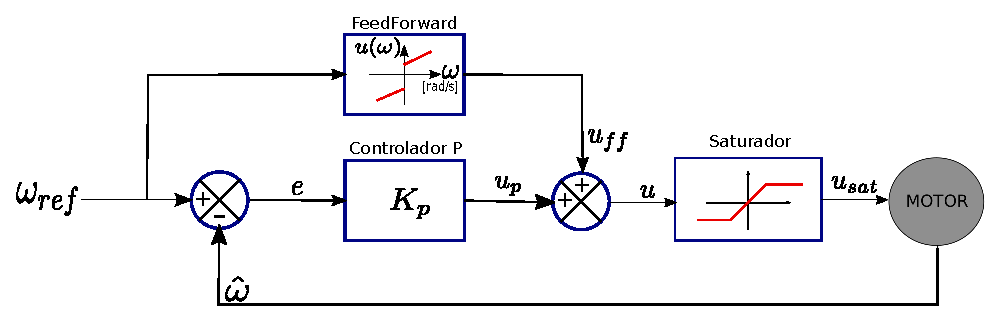
\includegraphics[width=\textwidth]{figuras/ilustracoes/sistema_de_controle_completo.eps}
    \caption{Diagrama de um sistema de controle \textit{Feedforward} + \textit{Backward}}
    \label{fig:diagrama_sistema_de_controle_feedforward_backward}
\end{figure}

\subsection{Sistemas de Primeira Ordem}

Um sistema de primeira ordem apresenta a seguinte forma genérica:

\begin{equation}
    T\dot{y} + y = Ku
\end{equation}

E em \emph{Laplace} com a seguinte função de transferência,

\begin{equation}
    G(s) = \frac{K}{Ts + 1}
\end{equation}

E sua resposta no tempo para uma entrada do tipo degrau unitário ($u(t) = 1 \xrightarrow{\mathscr{L}} U(s) = 1/s$),

\begin{equation}
    y(t) = K \left(1 - e^{-t/T} \right)
\end{equation}

Sendo $K$ o ganho do sistema e a constante $T$ é conhecida como constante de tempo do sistema e $T > 0$. A Figura \ref{fig:saida_sistema_primeira_ordem_no_tempo} ilustra o comportamento no tempo de um sistema de primeira ordem e a influência da constante de tempo $T$ na resposta do sistema.

\begin{figure}[H]
    \centering
    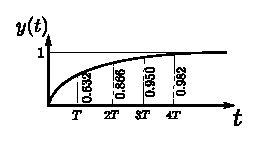
\includegraphics[width=0.7\textwidth]{figuras/ilustracoes/resposta_no_tempo_sistema_primeira_ordem.eps}
    \caption{Resposta no tempo ao degrau unitário de um sistema de primeira ordem com ganho unitário e contante de tempo $T$.}
    \label{fig:saida_sistema_primeira_ordem_no_tempo}
\end{figure}

% O erro de regime é a diferença entre os sinais de entrada e de saída na região de regime da resposta. Ou seja, $t \xrightarrow{} \infty$.
\section{Mínimos Quadrados}
De maneira geral, a ideia por trás do método dos mínimos quadrados (MMQ)  é de encontrar os coeficientes da(s) funções de base que minimizem o erro, ou seja, com o menor erro possível associado a representação \cite{MMQ}. Assim, dado que queremos obter a equação e possuímos vetores de dados $x$ e $y$, e queremos relacioná-los. Por exemplo, caso queira-se aproximar o conjunto de dados para a reta:

\begin{equation}
    y = ax + b.
    \label{eq:pol1}
\end{equation}

Teremos a seguinte relação para o MMQ.

\begin{align*}
    \textbf{Y} = \textbf{X}\alpha
\end{align*}
% \[\textbf{Y} = \textbf{X}\alpha\]
sendo,

\begin{equation*}
    \textbf{Y} =
    \begin{bmatrix}
     y_1\\
     y_2\\
     \vdots\\
     y_n
    \end{bmatrix},
    \textbf{X} = 
    \begin{bmatrix}
        x_1 & 1\\
        x_2 & 1\\
        \vdots & \vdots\\
        x_n & 1\\
    \end{bmatrix},
    \alpha =
    \begin{bmatrix}
        a\\
        b\\
    \end{bmatrix}
\end{equation*}

A ideia por trás do método de mínimos quadrados é minimizar o erro $e$. Sabendo que o espaço gerado por tal plano ortogonal será dado pela matriz $X^T$ , então queremos impor que o vetor
de erro $e$ será nulo, logo:

\[\textbf{X}^Te = 0\]

Como,

\[e = \textbf{Y} - \textbf{X}\hat{\alpha}\]

Então temos,

\[\textbf{X}^T(\textbf{Y} - \textbf{X}\hat{\alpha})= 0\]
\[\hat{\alpha} = (\textbf{X}^T\textbf{X})^{-1}\textbf{X}^T\textbf{Y} \]

Sendo,

\[\hat{\alpha} = 
\begin{bmatrix}
 \hat{a}\\
 \hat{b}\\
\end{bmatrix}
\]

Os elementos do vetor $\hat{\alpha}$, Serão os coeficientes da equação \ref{eq:pol1} que minimizarão o erro, ou seja, são os coeficientes da reta que melhor representa o conjunto de dados.
\section{Filtro de Kalman}
% Introdução ao filtro de Kalman
\label{sec:kalman}
"A filtragem de \emph{Kalman} é um processo de estimativa de estado ótimo aplicado a um sistema dinâmico que envolve perturbações aleatórias. Mais precisamente, o filtro de \emph{Kalman} fornece um  procedimento recursivo linear que visa minimizar a variância do erro para estimar de forma otimizada o estado desconhecido de um sistema dinâmico de dados ruidosos obtidos em tempo real discreto. Tem sido amplamente utilizado em muitas aplicações, como por exemplo, sistemas de rastreamento, navegação por satélite, estimar trajetória de mísseis balísticos e radar." \cite{kalman:book}.\\

O filtro de \emph{Kalman} usa um modelo dinâmico do sistema (por exemplo, leis físicas do movimento), entradas de controle conhecidas para esse sistema e várias medições sequenciais para formar uma estimativa das quantidades variáveis do sistema (seu estado $\textbf{x}_k$) que é melhor do que a estimativa obtida usando apenas as medições. Como tal, é um algoritmo comum de fusão de sensores e fusão de dados \cite{kalman:wiki}, \cite{Kalman:ofid}.\\

O filtro produz uma estimativa do estado do sistema como uma média do estado previsto do sistema e da nova medição usando uma média ponderada. O objetivo dos pesos é que os valores com menor incerteza sejam mais "confiáveis". O ganho de \emph{Kalman} é o peso relativo dado às medições e estimativa do estado atual.\\

Para o uso do filtro de \emph{Kalman} deve-se modelar o processo de acordo com a seguinte estrutura. Isso significa especificar as seguintes matrizes \cite{kalman:book}:

\begin{itemize}
    \item $\textbf{F}_k$: Modelo de transição de estado.
    \item $\textbf{H}_k$: Modelo de Observação.
    \item $\textbf{Q}_k$: Covariância do ruído do processo.
    \item $\textbf{R}_k$: Covariância do ruído da observação(medição).
    \item $\textbf{B}_k$: Modelo de entrada de controle (caso o sistema dinâmico tenha entrada). 
\end{itemize}


Modelo do sistema para o filtro de \emph{Kalman}:
\begin{equation}
\textbf{x}_k = \textbf{F}_x \textbf{x}_{k-1} + \textbf{B}_k \textbf{u}_k + \textbf{w}_k; \textbf{w}_k \sim N(0, \textbf{Q}_k)
\end{equation}

Sendo $\textbf{w}_k$ o ruído de processo, que assume-se ter uma distribuição normal de média zero e covariância $\textbf{Q}_k$. ($\textbf{w}_k \sim N(\textbf{0}, \textbf{Q}_k)$).

Modelo da observação/medição será:
\begin{equation}
\textbf{z}_k = \textbf{H}_k \textbf{x}_k + \textbf{v}_k; \textbf{v}_k \sim N(\textbf{0}, \textbf{R}_k)
\end{equation}

Sendo $\textbf{v}_k$ o ruído de observação, que assume-se ser um ruído gaussiano branco de média zero e covariância $\textbf{R}_k$. ($\textbf{v}_k \sim N(\textbf{0}, \textbf{R}_k)$).

A filtragem é frequentemente dividida em duas fases: Predição e atualização (Alguns autores também contam a etapa de medição como uma fase do algoritmo). A fase de predição usa a estimativa anterior para produzir uma estimativa do estado atual. Na fase seguinte (de atualização), a predição atual é combinada com as informações da medição atual para aprimorar a estimativa do estado. As etapas do filtro são apresentadas a seguir.

\textbf{Predição}:
\begin{align*}
    \check{\textbf{x}}_k &= \textbf{F}_k \hat{\textbf{x}}_{k-1} + \textbf{B}_k \textbf{u}_k\\
    \check{\textbf{P}}_k &= \textbf{F}_k \hat{\textbf{P}}_{k-1} \textbf{F}^T_k + \textbf{Q}_k
\end{align*}

Sendo $\check{\textbf{P}}$ uma predição da covariância do estado seguinte (predito, $\textbf{x}_k$).

\textbf{Atualização}:
\begin{align*}
    \textbf{K}_k &= \check{\textbf{P}}_k \textbf{H}^T \left( \textbf{H}_k \check{\textbf{P}}_k \textbf{H}^T_k + \textbf{R}_k\right)^{-1}\\
    \hat{\textbf{x}}_k &= \check{\textbf{x}}_k + \textbf{K}_k\left( \textbf{z}_k - \textbf{H}_k \check{\textbf{x}}_k \right)\\
    \hat{\textbf{P}}_k &= \left(\textbf{I} - \textbf{KH}_k \right)\check{\textbf{P}}_k
\end{align*}

Uma observação importante sobre a etapa de atualização é que o valor atualizado irá tender para o valor predito caso o ganho do filtro $\textbf{K}_k$ seja baixo (resultado de um alto erro na medição). O contrário também ocorre, ou seja, para medições precisas ($\textbf{R}_k$ baixo) o ganho do filtro tende a ser alto e a etapa de atualização vai tender a usar mais a informação da medição na estimação do estado ótimo ($\hat{\textbf{x}}$). 

\section{\textit{Encoders} Incrementais}
% Referencias:
% https://www.roboticsbusinessreview.com/news/differences-between-encoder-resolution-accuracy-and-precision/
% https://www.newtoncbraga.com.br/index.php/como-funciona/5454-mec128
% [Speed Measumment Using Rotary Encoders for High Performance ac Drives]
% [Speed Measurement Algorithms for Low-Resolution Incremental Encoder Equipped Drives: a Comparative Analysis]
% [A Simple Speed Feedback System for Low Speed DC Motor Control in Robotic Applications]
% [An Embedded System for Position and Speed Measurement Adopting Incremental Encoders]

% FALAR SOBRE O FUNCIONAMENTO BASICO
% CITAR OS DIFERENTES TIPOS
% FALAR DO GRAY CODE
% FALAR DO ERRO DE QUANTIZAÇÃO

As saídas de um \emph{Encoder} incremental são, normalmente, duas ondas quadradas defasadas em $90^\circ$ uma da outra (em quadratura). Essa diferença de fase nos permite medir o sentido de rotação. Abordagens mais eficientes de leitura desses sensores é por meio da detecção das bordas dessas ondas, pois isso permite quadruplicar o número de pulsos por revolução (NPR) \cite{quantization_error01}. Existem dois métodos básicos para se realizar a medição da velocidade por meio desses sensores, são eles: \textbf{frequencímetro} e \textbf{periodímetro}. 

Na medição por frequência (\textbf{frequencímetro}), conta-se o número de pulsos que ocorreram em um determinado período de tempo fixo. Com isso a velocidade pode ser obtida pela seguinte aproximação:

\begin{equation}
    \omega = \frac{d\theta}{dt} \cong \frac{\Delta{\theta}}{T} \cong \frac{2 \pi \Delta{N}}{N_{PR}T}[rad.s^{-1}] \xrightarrow{} \frac{60 \Delta{N}}{N_{PR} T} [RPM]
\end{equation}

Sendo $N_{PR}$ o número de pulsos por revolução e $\Delta{N}$ é o número de pulsos que aconteceram dentro da janela de tempo $T$. Existe um erro de quantização nesse método de leitura devido a variação de ângulo medida ser sempre um múltiplo inteiro de $ 2\pi/N_{PR}$. O erro de quantização $\Delta{\omega}$ pode ser modelado pela seguinte equação:

\begin{equation}
    \Delta{\omega} = \frac{2\pi}{N_{p}T}[rad.s^{-1}] \xrightarrow{} \frac{60}{N_{PR}T}[RPM]
    \label{eq:erro_de_quantizacao_frequencimetro}
\end{equation}

\begin{figure}[H]
    \centering
    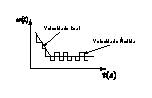
\includegraphics[width=0.5\textwidth]{figuras/ilustracoes/ilustracao_erro_de_quantizacao.eps}
    \caption{Ilustração do erro de quantização na medição de velocidade de rotação.}
    \label{fig:ilustracao_erro_quantizacao}
\end{figure}

A Figura \ref{fig:ilustracao_erro_quantizacao} ilustra um exemplo de medição de velocidade com erro de quantização.\\

Nota-se pela Equação \ref{eq:erro_de_quantizacao_frequencimetro} que o erro de quantização para a medição por frequência decresce com o aumento do número de pulsos por revolução e/ou com o aumento da janela de tempo ($T$), porém o aumento do período de observação acrescenta um atraso na medição da velocidade. O erro relativo à velocidade pode ser descrito como a seguir:

\begin{equation}
    e_{\omega} = \frac{2\pi}{\omega N_{PR} T}
    \label{eq:erro_relativo_quantizacao_frequencimetro}
\end{equation}

Pela Equação \ref{eq:erro_relativo_quantizacao_frequencimetro} observa-se que o erro relativo decresce conforme a velocidade $\omega$ aumenta, ou seja, o erro de quantização será mais significante para baixas velocidades.\\

O outro método de leitura dos \emph{Encoders} incrementais é por medição de intervalos de tempo de um mesmo pulso (\textbf{periodímetro}) (ver Figura \ref{fig:ilustracao_periodimetro}). A seguinte formulação pode ser obtida considerando a velocidade do motor constante e sem levar em conta o sentido de giro:

\begin{equation}
    \omega = \frac{d\theta}{dt} \cong \frac{\Delta{\theta}}{nT_{hf}} \cong \frac{2\pi}{N_{PR} n T_{hf}} [rad.s^{-1}] \xrightarrow{} \frac{60}{N_{PR} n T_{hf}} [RPM]
    \label{eq:omega_periodimetro}
\end{equation}

O período entre pulsos será:

\begin{equation}
    T_{\omega}(\omega) = \frac{2\pi}{N_{p}\omega} [s]
\end{equation}

Uma aproximação para o pior caso do erro de quantização relativo a velocidade é apresentado a seguir \cite{analise_incr_enc}:

\begin{equation}
    e_{\omega} = \frac{T_{hf}}{ \frac{2\pi}{N_{PR} \omega} - T_{hf} } \cong \frac{\omega N_{PR} T_{hf}}{2\pi}
    \label{eq:erro_quantizacao_periodimetro}
\end{equation}

A Equação \ref{eq:erro_quantizacao_periodimetro} mostra que o erro é diretamente proporcional à velocidade e a quantidade de pulsos por revolução ($N_{PR}$) e decresce com o aumento da frequência do contador de alta frequência (diminuição de $T_{hf}$).


\begin{figure}[H]
    \centering
    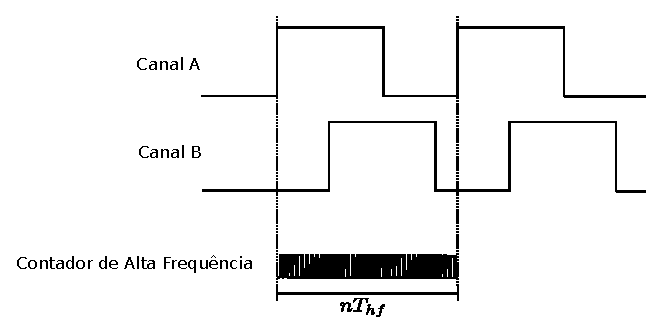
\includegraphics[width=0.5\textwidth]{figuras/ilustracoes/ilustracao_medicao_encoder_por_periodo.eps}
    \caption{Ilustração de leitura de \emph{Encoder} periódica.}
    \label{fig:ilustracao_periodimetro}
\end{figure}

Já para se obter o \textbf{sentido da velocidade $\omega$} é necessário fazer uso do padrão binário gerado pelas bordas dos sinais em quadratura. A Figura \ref{fig:cw_signal} ilustrado os sinais em quadratura para uma rotação no sentido horário e destaca o padrão binário gerado nas bordas. A Figura \ref{fig:ccw_signal} ilustra os sinais no sentido anti-horário. O padrão de dois bits é apresentado na Tabela \ref{tab:tabela_simple_code}. \\

\begin{figure}[H]
    \centering
    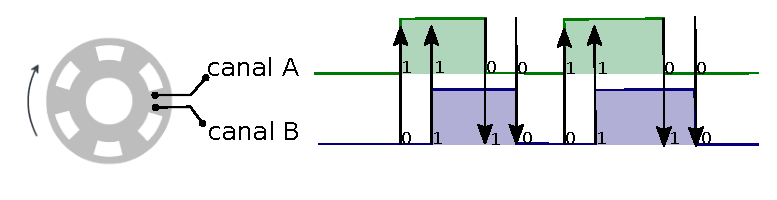
\includegraphics[width=0.7\textwidth]{figuras/ilustracoes/sinal_enquadratura_sentido_CW.eps}
    \caption{Sinal em quadratura para rotação no sentido horário.}
    \label{fig:cw_signal}
\end{figure}

\begin{figure}[H]
    \centering
    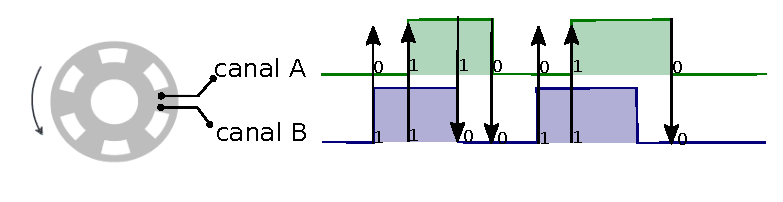
\includegraphics[width=0.7\textwidth]{figuras/ilustracoes/sinal_enquadratura_sentido_CCW.eps}
    \caption{Sinal em quadratura para rotação no sentido anti-horário.}
    \label{fig:ccw_signal}
\end{figure}

% Please add the following required packages to your document preamble:
% \usepackage{graphicx}
\begin{table}[H]
\centering
\resizebox{0.5\textwidth}{!}{%
\begin{tabular}{cc|cc}
\multicolumn{2}{c|}{\textbf{\begin{tabular}[c]{@{}c@{}}Sentido\\     Horário\end{tabular}}} &
  \multicolumn{2}{c}{\textbf{\begin{tabular}[c]{@{}c@{}}Sentido\\ Anti-Horário\end{tabular}}} \\ \hline
\textbf{A} & \textbf{B} & \textbf{A} & \textbf{B} \\
1          & 0          & 0          & 1          \\
1          & 1          & 1          & 1          \\
0          & 1          & 1          & 0          \\
0          & 0          & 0          & 0         
\end{tabular}%
}
\caption{Código de 2 bits para identificar o sentido de rotação.}
\label{tab:tabela_simple_code}
\end{table}


\begin{comment}
% Speed Measumment Using Rotary Encoders
% for High Performance ac Drives

SPEED MEASUREMENT USING A PERIODIMETER

If we use a periodimeter, we will get the speed not by counting pulses from the encoder, but by counting a high frequency (HF) clock

Let $\alpha_p$ be the corresponding angle to the higher part of an encoder pulse (half of its period), t the period of the HF clock, and n the number of HF pulses arrived at the HF counter. Then, the time spent on an encoder pulse, $T_e$ is:

\begin{equation}
    T_e = n t
\end{equation}

Rotor speed can be obtained as:

\begin{equation}
    \omega_{rotor} = \frac{\alpha_p}{T_e}
\end{equation}

As with the frequencimeter, here also there is a quantization error because of the time T,, which will be always an integer multiple of t With a fixed HFclock frequency, this error will increase as n decreases, that is, as the encoder rotates faster, but it provides accurate measurements at lower speeds. Because the variable with quantization noise is now in the denominator, its effects are much more important than in the frequencimeter.

An additional advantage at low speed is that, as it only needs one pulse to get the speed, the delay is minimal, which is very important at lower speeds.

It also possible to use quadruple frequency. Of course, this reduces the precision, and therefore the maximum velocity where this method is suitable, but also, and this is much more important, it reduces the delay obtaining the velocity when the motor works at low speed. Nevertheless, this method produces stability problems in the zero speed cross. Figure 8 shows an inversion with two possible situations in the encoder output signals. Supposing that there is no quadruple frecuency, and PHASE A controls the HF counter, we see that at the encoder pulse end, the counter has a wrong value, because about half of the HF pulses arrived on each direction of rotation.

The accuracy of the periodimeter is, more than the frequencimeter, related to the accuracy of the encoder, which in general depends on the errors in the radial grating, and the eccentricity of the graduated disk to the bearing.

% Speed Measurement Algorithms for
% Low-Resolution Incremental Encoder Equipped
% Drives: a Comparative Analysis


At very low speed the number of high frequency pulses can be extremely high and saturation of the digital timer employed for measurement can occur. Also a speed sample is not available each speed control period, needing an adaptation of the control parameters. In that situation, the quadrature decoding of the encoder pulses can be exploited in order to reduce the width of the measuring window by a factor of four or a reduction of the frequency of the timer can be considered.

The former solution allows to reduce the speed sampling period and improve the control performance of the drive, but makes the measuring system more sensitive to sensor nonidealities, including variations in the transition locations from their nominal values and phasing errors between encoder channels. When low-cost and low-resolution sensors are employed, nonidealities play the major role in the determination of period measuring errors and has to be carefully analysed in drive design phase. The latter solution needs to switch on-line the frequency of the timer and adapt the coeffients of the equations above.

The implementation of the period measuring method is also straightforward as it requires a simple timer capture unit, commonly found inside recent microcontrollers.

% A Simple Speed Feedback System for Low Speed
% DC Motor Control in Robotic Applications

The relationship between the measured frequency using PIC microcontroller and the percentage error is shown in Fig. 2. The percentage error is given as:

\begin{equation}
    e\% = \frac{F_m - F_a}{F_a}.100
\end{equation}

where F m and F a denote the measured and actual frequencies. It is observed that as the frequency increases, the error in the frequency measured from PIC increases linearly, that is, there is a linear relationship between error and frequency.

\end{comment}
\section{Bluetooth}
\label{sec:bluetooth}
% Breve introdução à historia do bluetooth e utilidade
% destacar: custo energético, velocidade de operação, robustez a interferências
A  tecnologia \emph{Bluetooth}  suporta várias opções de topologia, incluindo conexões simples ponto a ponto. Operando na faixa de frequência industrial, científica e médica de $2,4$ GHz, a tecnologia \emph{Bluetooth} suporta várias opções de rádio.

O rádio \emph{Bluetooth} BR/EDR opera com baixo consumo de energia e também utiliza uma abordagem robusta de \textit{Adaptive Frequency Hopping}, transmitindo dados por $79$ canais. O \textit{Bluetooth} BR/EDR inclui várias opções de configuração para a camada física (\emph{PHY}) que suportam taxas de dados de $1$ Mb/s a $3$ Mb/s e suporta vários potências de transmissão, de $1$ mW a $100$ mW, além de várias opções de segurança.
% aprofundar mais? 
\section{Modulação por Largura de Pulso}
\label{sec:PWM}
% Resumo sobre PWM

\emph{Pulse Width Modulation} (PWM) refere-se a um sinal digital pulsante. Esse sinal é utilizado, por exemplo, para simular uma saída analógica em microcontroladores e por isso geralmente é muito usado para o controle de atuadores elétricos como motores, aquecedores, dentre outras coisas, como o controle do brilho de LEDs. \\

A modulação \emph{PWM} pode ser vista como uma maneira de codificar digitalmente níveis de sinal analógico. Nesta técnica, através do uso de contadores de alta resolução, o ciclo de trabalho de uma onda quadrada é modulado para codificar um nível de sinal analógico específico para que então ele atenda os requisitos de uma aplicação desejada. O tempo de ativação é o tempo durante o qual a alimentação CC é aplicada (sinal em nível alto) à carga e o tempo de desativação é o período durante o qual a alimentação é desligada (sinal em nível baixo). Dada uma largura de banda suficiente, qualquer valor analógico pode ser codificado com \emph{PWM}.

% Metodologia
\chapter[Metodologia]{Metodologia}
\label{ch:metodologia}

Nessa seção será apresentado de forma técnica e descritiva a metologia utilizada para as implementações do sistema de controle, do observador/estimador de velocidade (filtro de \emph{Kalman}), dentre outras implementações que foram relevantes para o trabalho. Além disso será apresentado os componentes utilizados, bem como todo o projeto do robô desenvolvido durante o trabalho, que serviu como aplicação alvo para a validação do trabalho.

% Apresentação e descrição dos componentes utilizados
% Projeto estrutural e eletrônico
\section{Os Robôs}
A estrutura dos robôs utilizados foi projetada em \emph{software} CAD e impressa com o uso de impressão 3D de forma a possuírem uma base quadrada de 7.5cm de lado e 6.5cm de altura contando com o raio das rodas que é de 3cm. A Figura \ref{fig:robo_completo_explodido} apresenta uma imagem do modelo 3D do robô.\\

\begin{figure}[H]
    \centering
    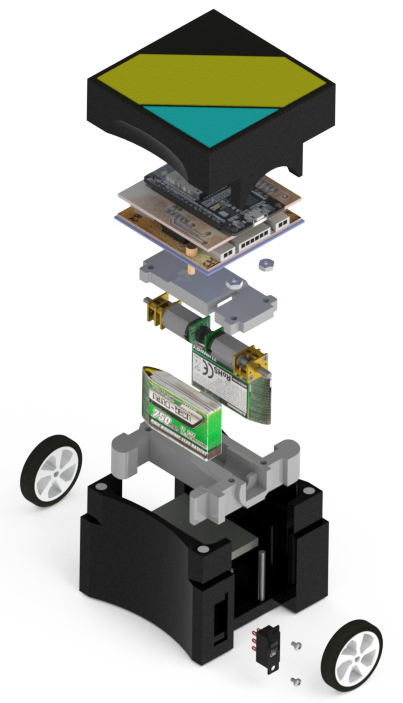
\includegraphics[width=0.5\textwidth]{figuras/robo/robo_completo_explodido.png}
    \caption{Vista explodida do robô completo.}
    \label{fig:robo_completo_explodido}
    \fonte{Victor Duarte de Queiroz (não publicada).}
\end{figure}

\begin{figure}[H]
    \centering
    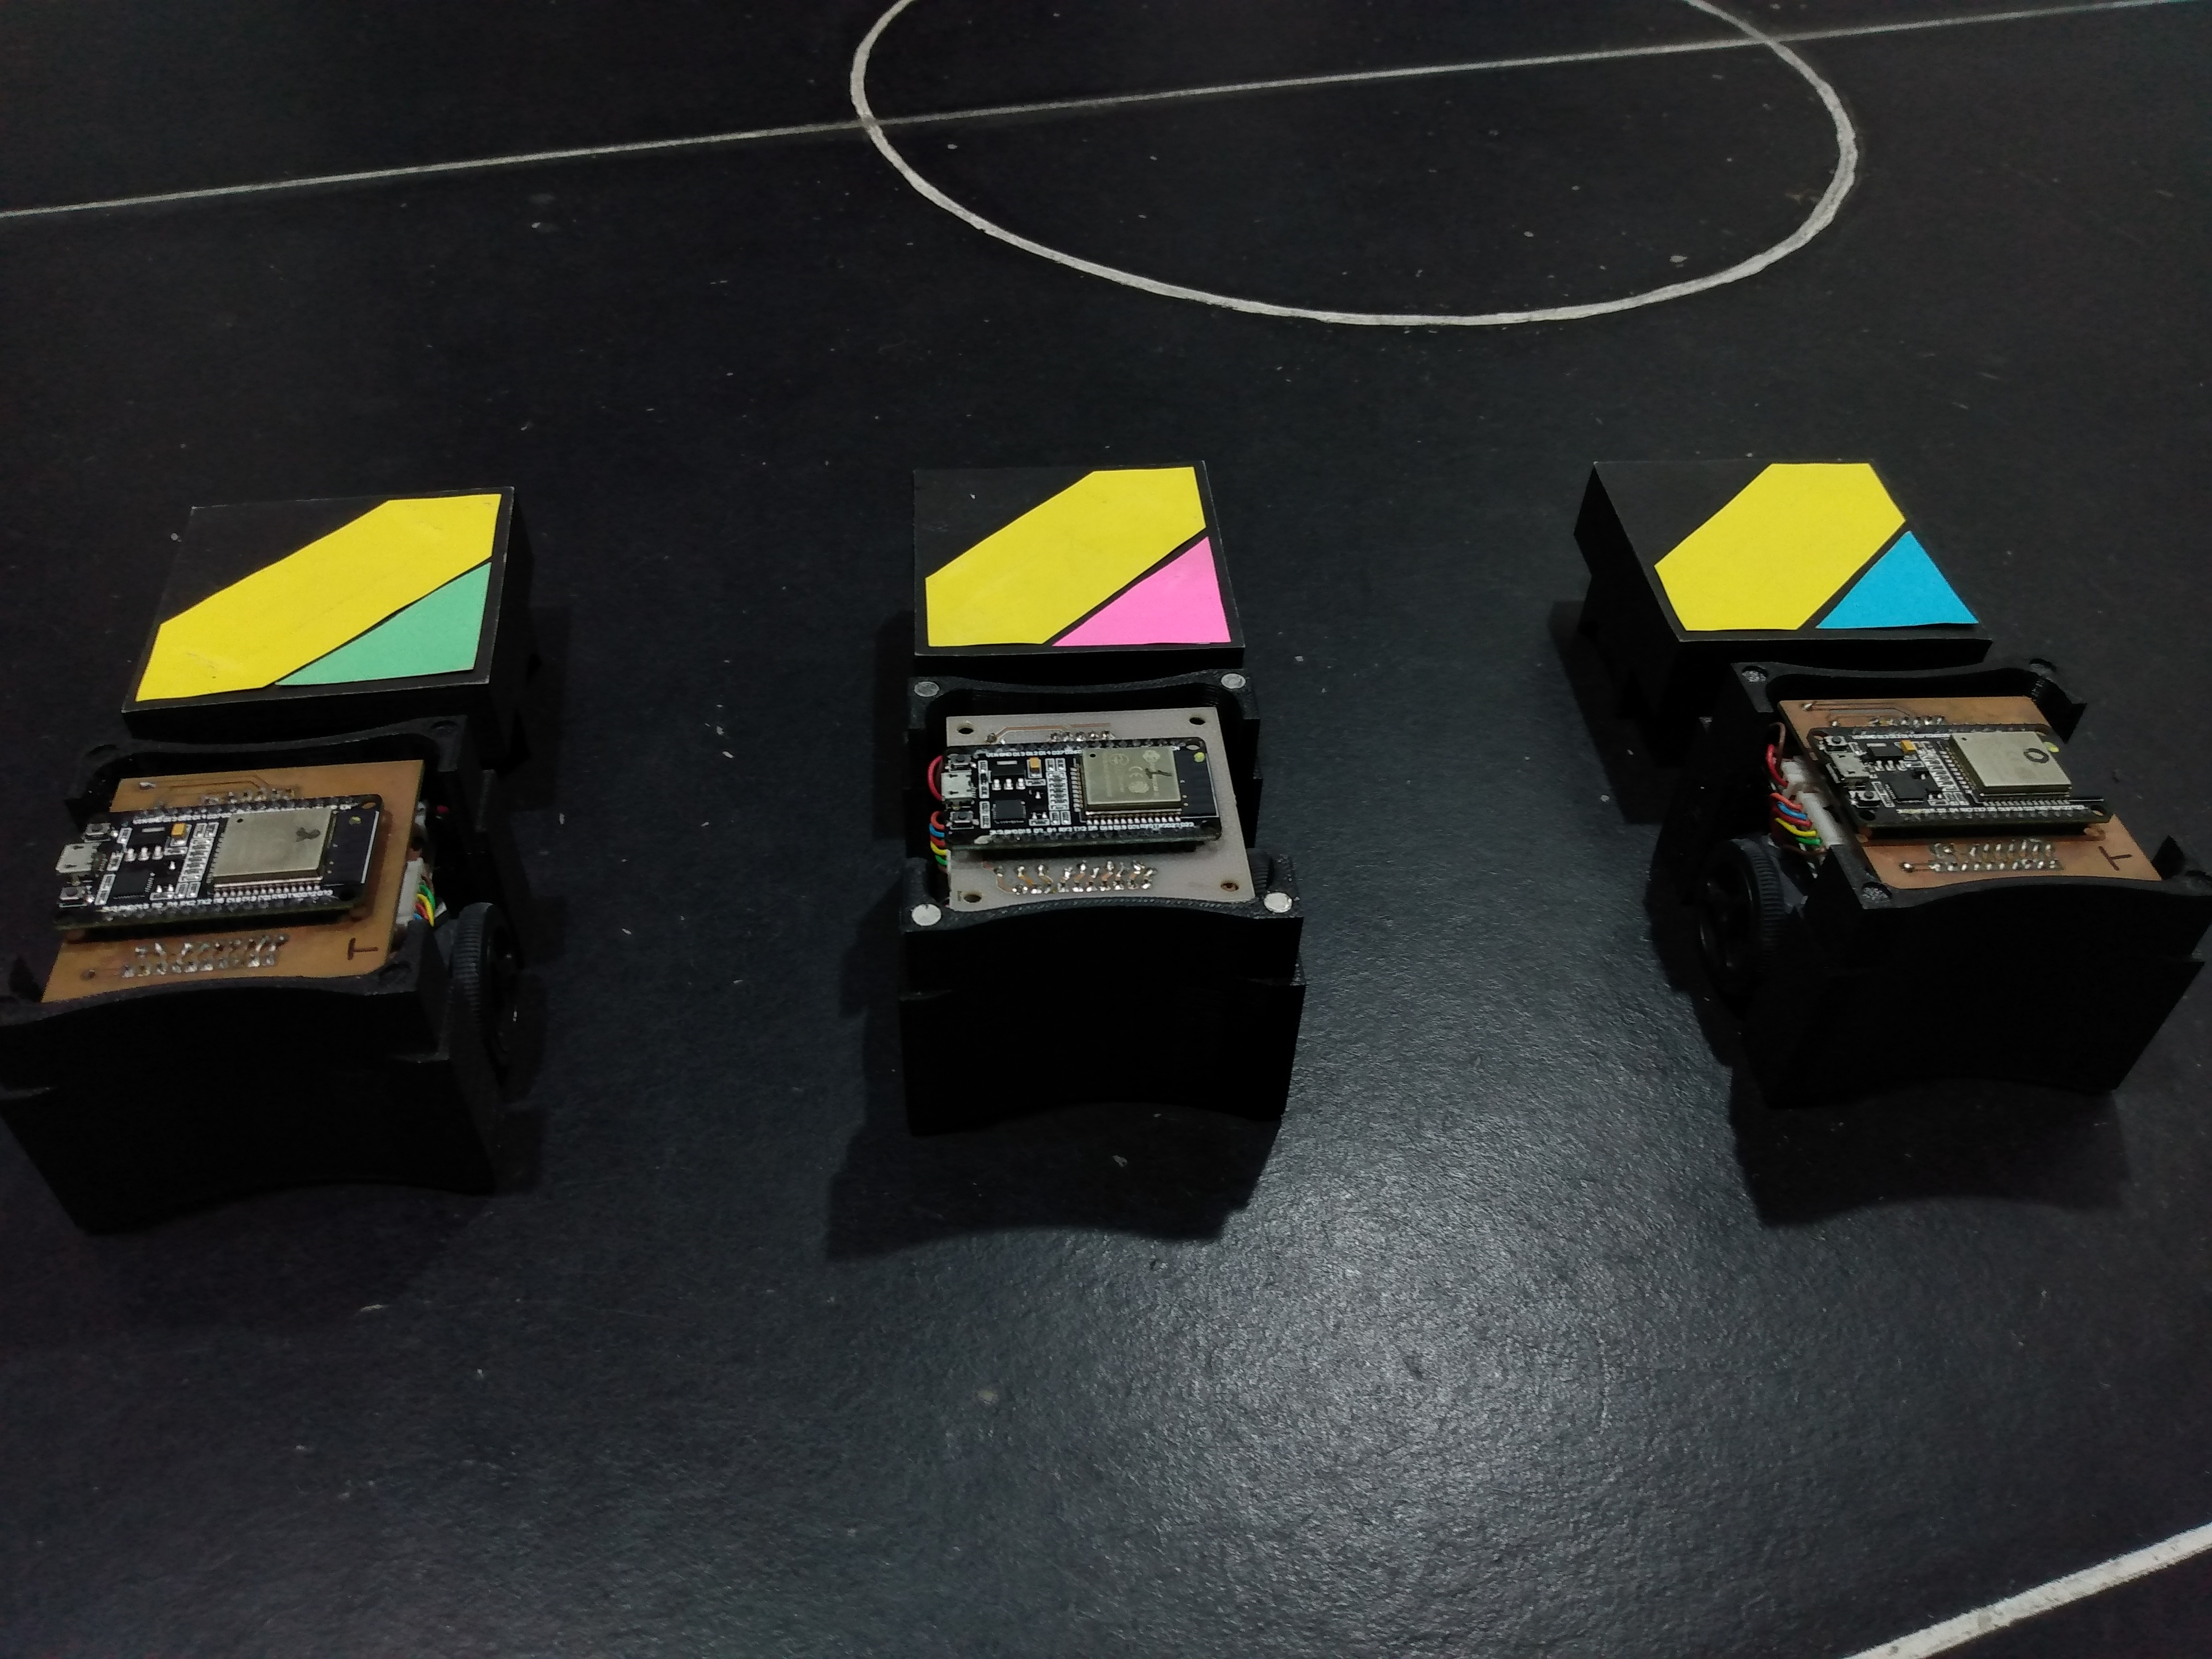
\includegraphics[width=0.5\textwidth]{figuras/robo/robos_capa_aberta.jpg}
    \caption{Frota de mini robôs da Equipe Poti de Futebol de robôs.}
    \label{fig:robos_capa_aberta}
    \fonte{Própria.}
\end{figure}

Já a Figura \ref{fig:robos_capa_aberta} mostra três dos robôs reais (um time) projetados, desenvolvido pela equipe Poti. As subseções seguintes apresentam mais detalhes a respeito do projeto desses robôs.

\subsection{Componentes}
% Motor: 
% https://www.pololu.com/product/2212
% https://www.pololu.com/product/2212
% Encoder:
% https://www.pololu.com/product/3081
% Driver motor:
% https://www.pololu.com/product/713
% ESP32:

São quatro o número de componentes básicos que compõem os robôs presentes neste trabalho, sendo eles: um par de atuadores (motor direito e esquerdo), um par de sensores de rotação (\textit{Encoder}s magnéticos), um driver motor multicanal, um microcontrolador e bateria recarregável. Devido as características dos componentes escolhidos para o projeto, apenas estes quatro tipos foram suficiente para compor a eletrônica do robô de forma a respeitar as restrições dimensionais, realizar o controle feedforward/backward de forma eficiência e com um bom período de amostragem e baixo gasto energético, além de um baixo custo financeiro.

A seguir serão apresentados mais detalhes dos componentes supracitados.

% 30:1 Micro Metal Gearmotor HP 6V with Extended Motor Shaft
\begin{figure}[H]
    \centering
    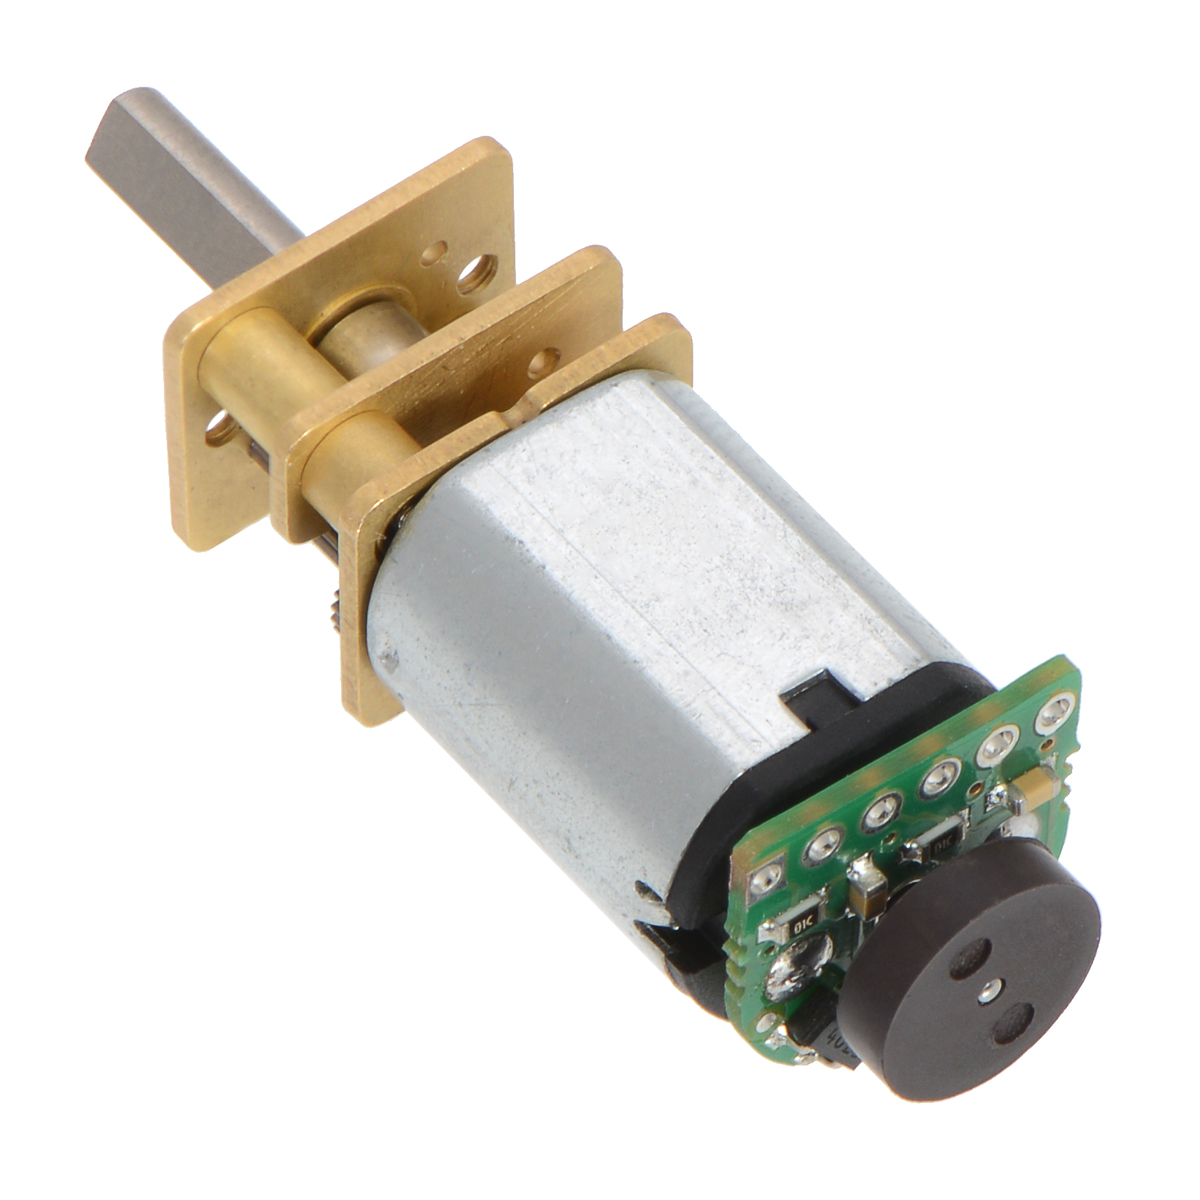
\includegraphics[width=3cm]{figuras/eletronica/motor_com_encoder.jpg}
    \caption{Micro Motor de 6V com caixa de redução de 30:1 e \textit{Encoder} magnético.}
    \label{fig:motor_com_encoder}
\end{figure}

A figura \ref{fig:motor_com_encoder} mostra o motor escolhido já com o \textit{Encoder} magnético colocado em seu eixo estendido (placa de circuito impresso com um Imã natural em forma de disco), esse é um micro motor de $6$V com uma caixa de redução de $\approx 30:1$ da \textit{Pololu}[?].

\begin{figure}[H]
    \centering
    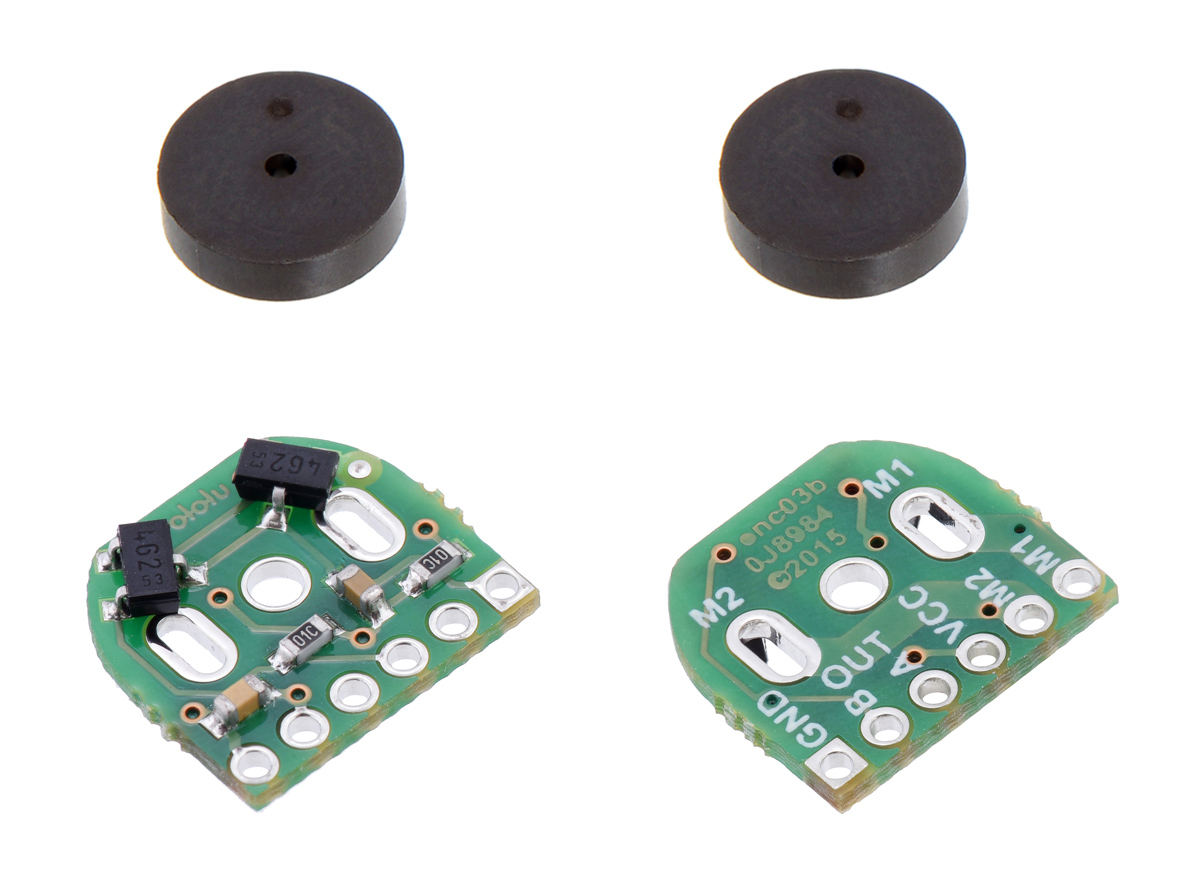
\includegraphics[width=5cm]{figuras/eletronica/encoder_frente_verso.jpg}
    \caption{Par de Encoders Magnéticos de $12$ pulsos por revolução ($12$CPR)}
    \label{fig:encoder}
\end{figure}

\begin{figure}[H]
    \centering
    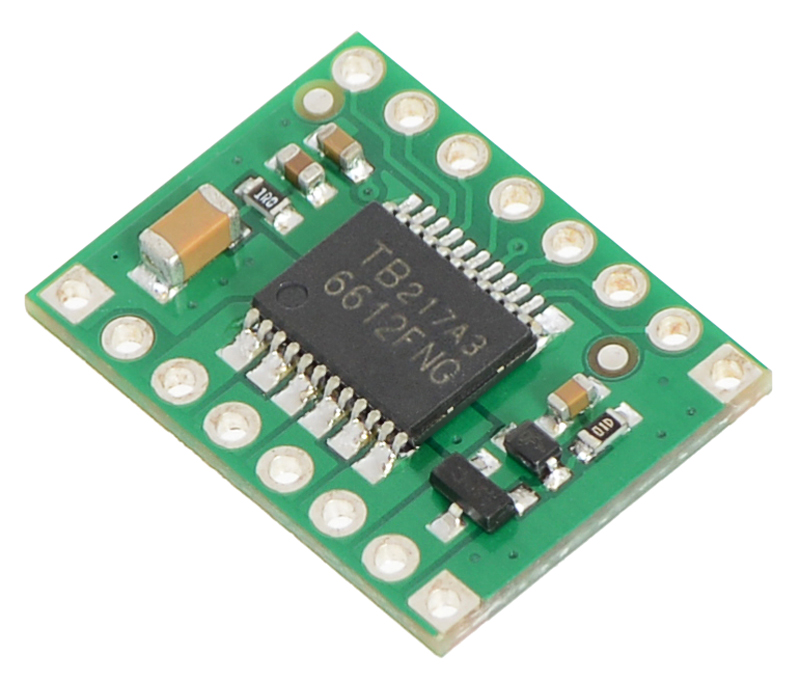
\includegraphics[width=3cm]{figuras/eletronica/driver.jpg}
    \caption{\textit{Driver} Motor TB6612FNG.}
    \label{fig:driver_motor}
\end{figure}

\begin{figure}[H]
    \centering
    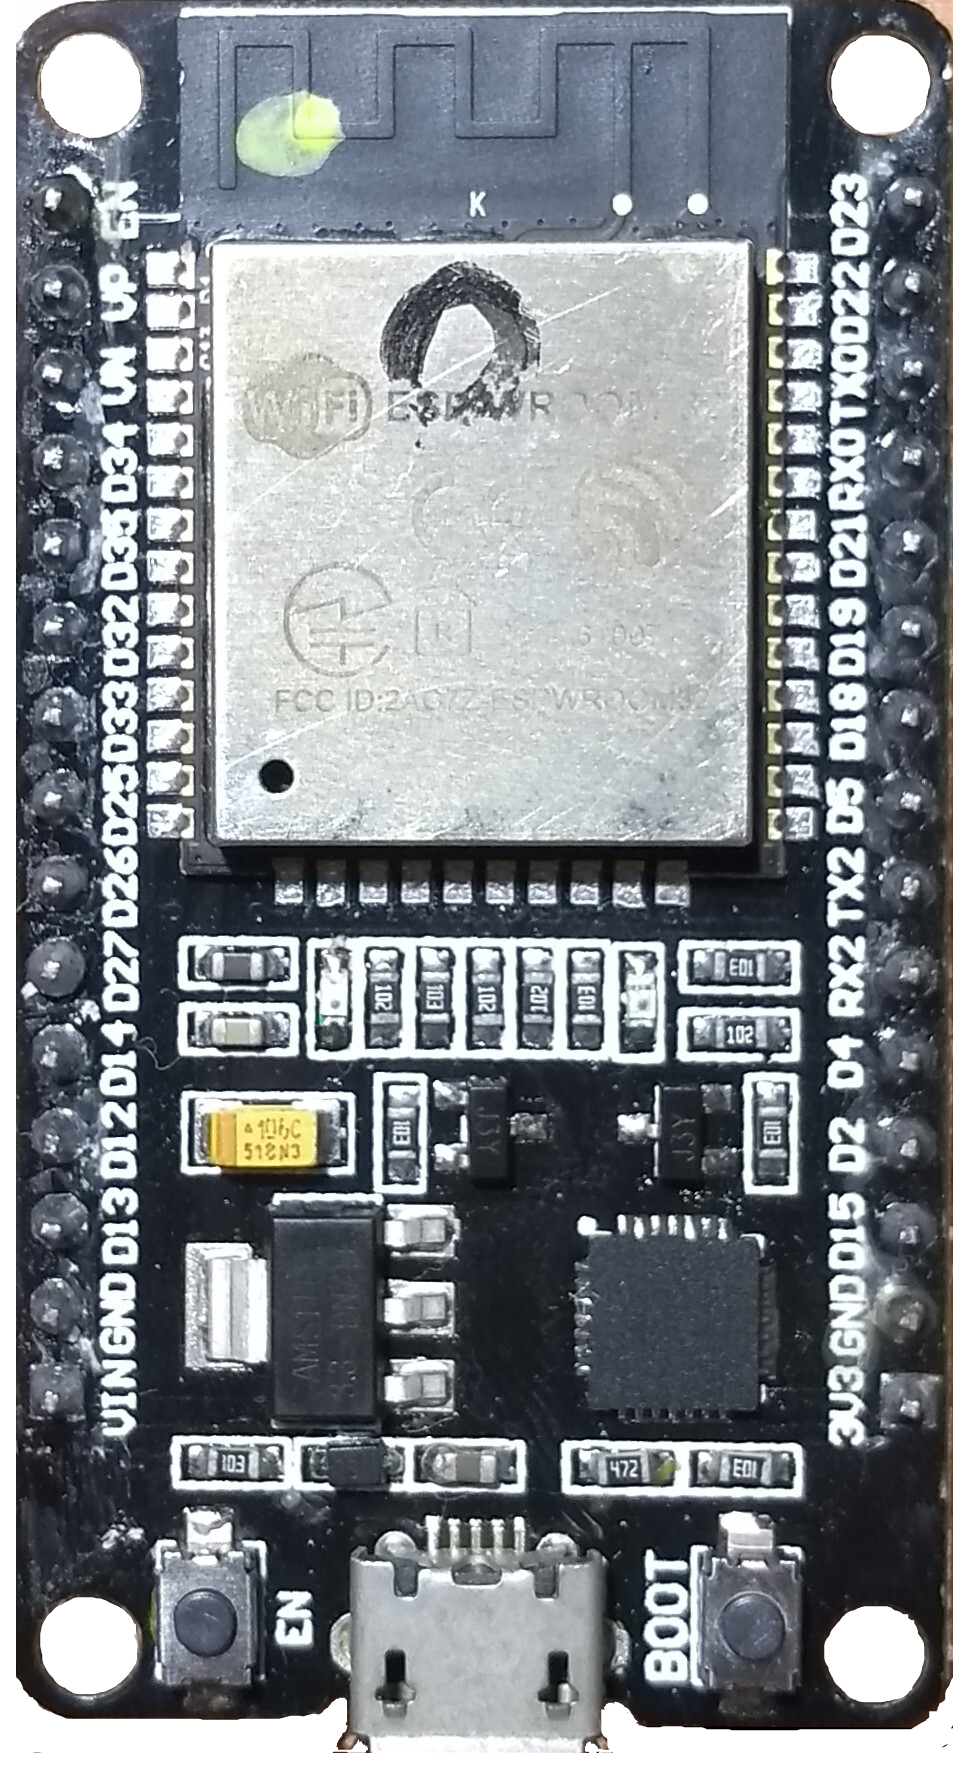
\includegraphics[width=3cm]{figuras/eletronica/esp32_kit.png}
    \caption{Placa de desenvolvimento ESP32 Dev1.}
    \fonte{Própria}
    \label{fig:esp32_kit}
\end{figure}
\subsection{Projeto Eletrônico}
% CIRCUITO ELÉTRICO/ELETRÔNICO COMPLETO
% MOSTRAR/EXPLICAR: PLACA DE CIRCUITO IMPRESSO DESENVOLVIDA
% TODO:
% ref:  https://produza.ind.br/gestao/pre-requisitos-tecnicos-para-montar-um-projeto-eletronico/

% \begin{figure}[H]
%     \centering
%     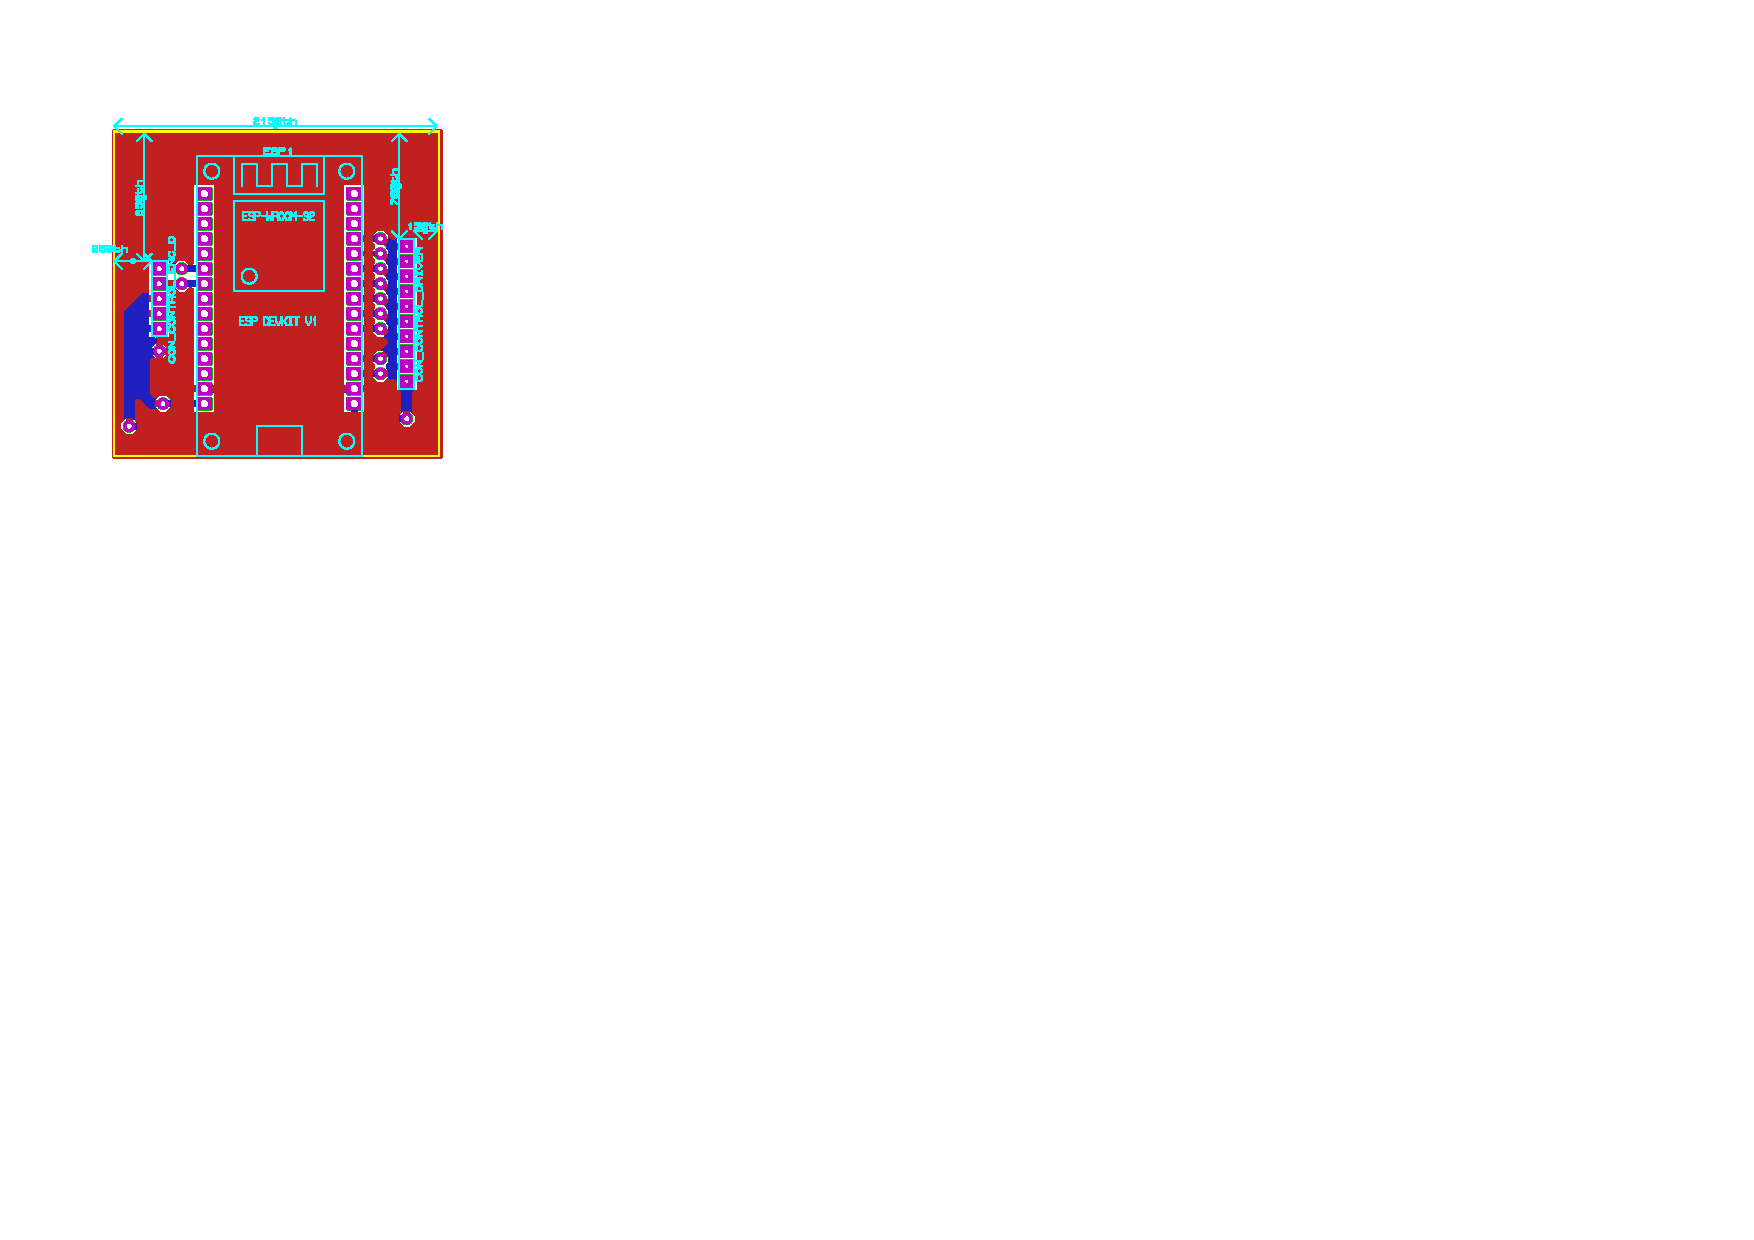
\includegraphics[width=\textwidth]{imagens/eletronica/placa/placa_controle_completa.pdf}
%     \caption{Caption}
%     % \label{fig:my_label}
% \end{figure}

% \begin{figure}[H]
%     \centering
%     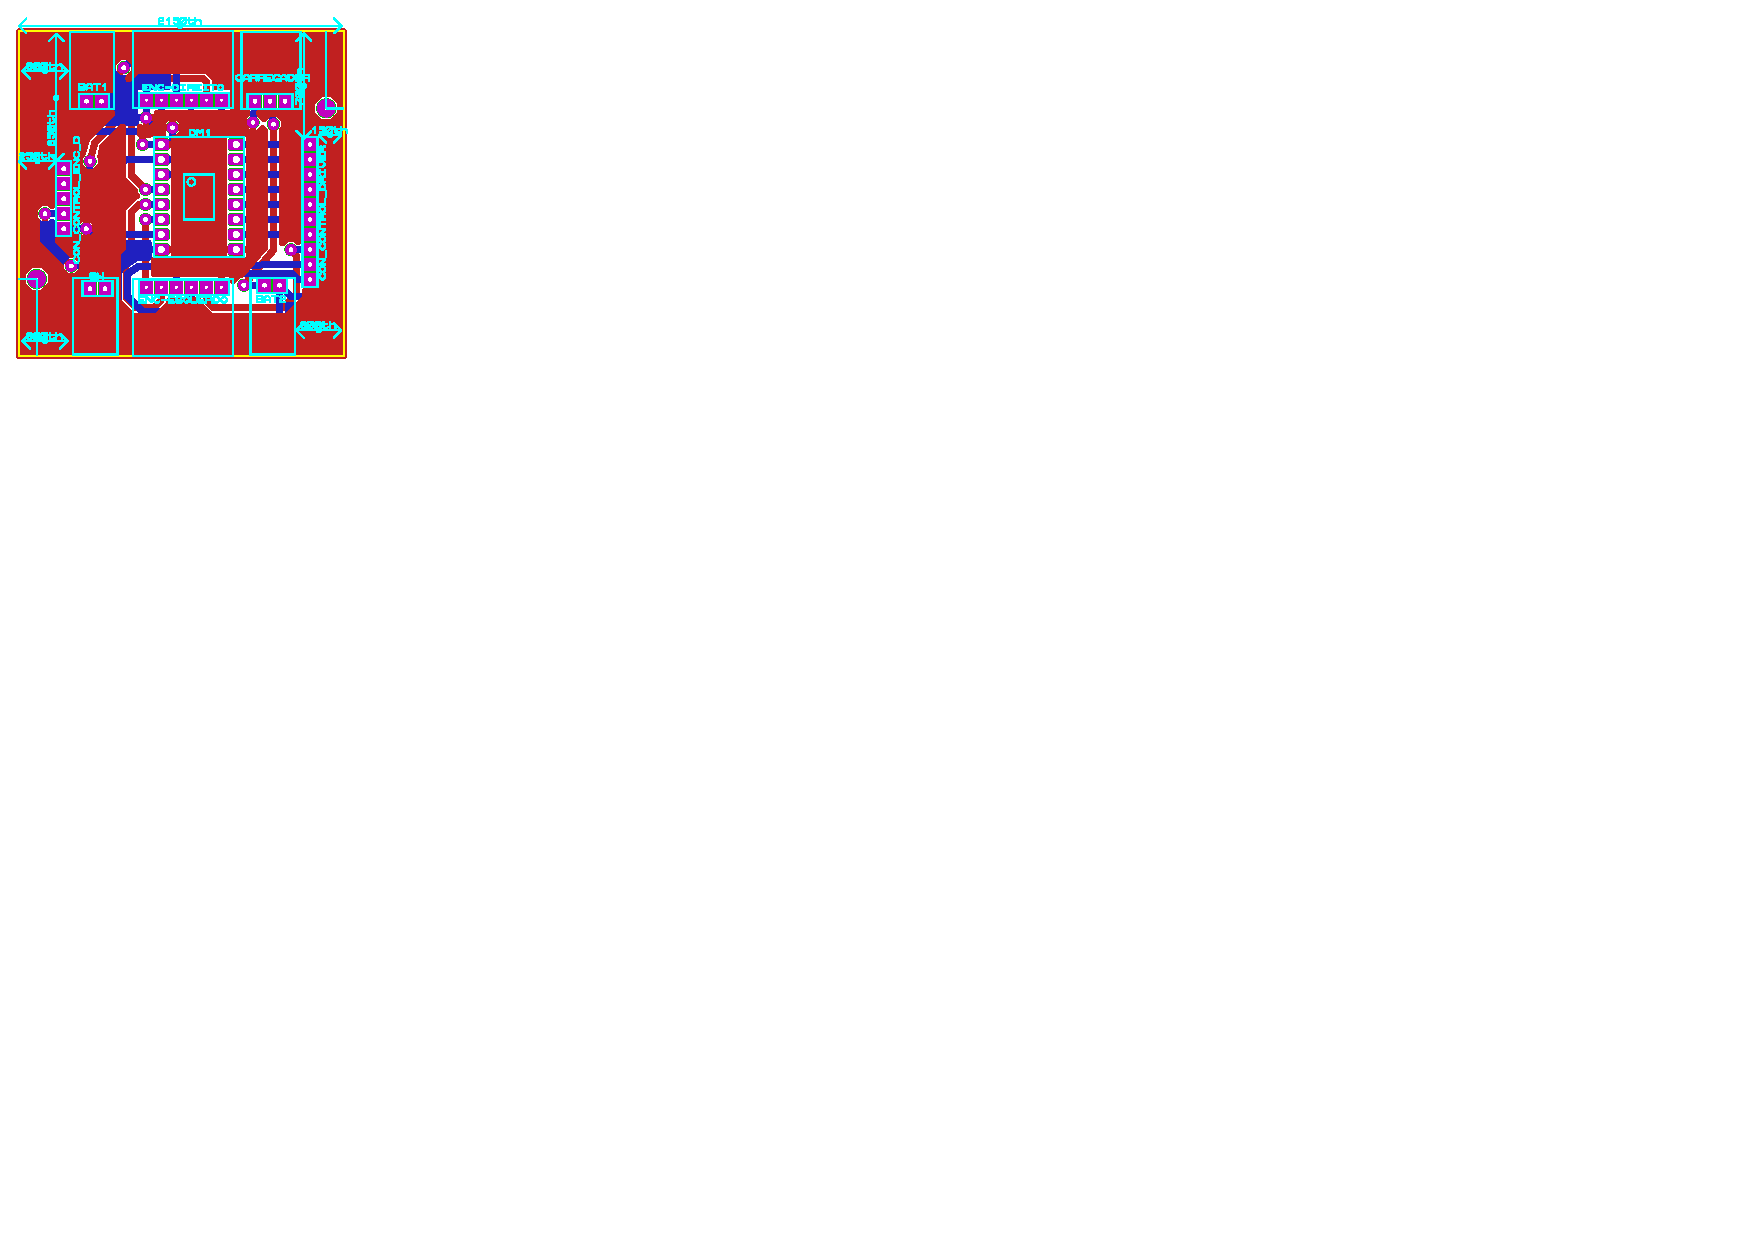
\includegraphics[width=\textwidth]{imagens/eletronica/placa/placa_driver_completa.pdf}
%     \caption{Caption}
%     % \label{fig:my_label}
% \end{figure}

\begin{enumerate}
    \item \textbf{Concepção inicial}:
        O principal objetivo por trás de se fazer uma nova placa de circuito eletrônico é acomodar os componentes, respeitando os limites das dimensões estabelecidos pela competição na qual os robôs serão utilizados (caber dentro de um cubo de $75$ mm de aresta). A placa deve conter o microcontrolador, no seu kit de desenvolvimento, \textit{Driver motor} para acionamento dos motores DCs, os \textit{Encoders} e ser alimentada por duas baterias de $1$ célula do tipo \textit{Lipo}.
        
    \item \textbf{Elaboração dos esquemáticos eletrônicos}:
        O esquemático foi a parte mais simples, pois não houve grandes mudanças nessa parte, com relação aos projetos de anos anteriores. A maior mudança foi o microcontrolador, que provocou dificuldades maiores na etapa seguinte, a elaboração do \textit{Layout}, devido às dimensões dos componentes.
        
        % inserir imagem do esquemático geral aqui
        
        \begin{figure}[H]
            \centering
            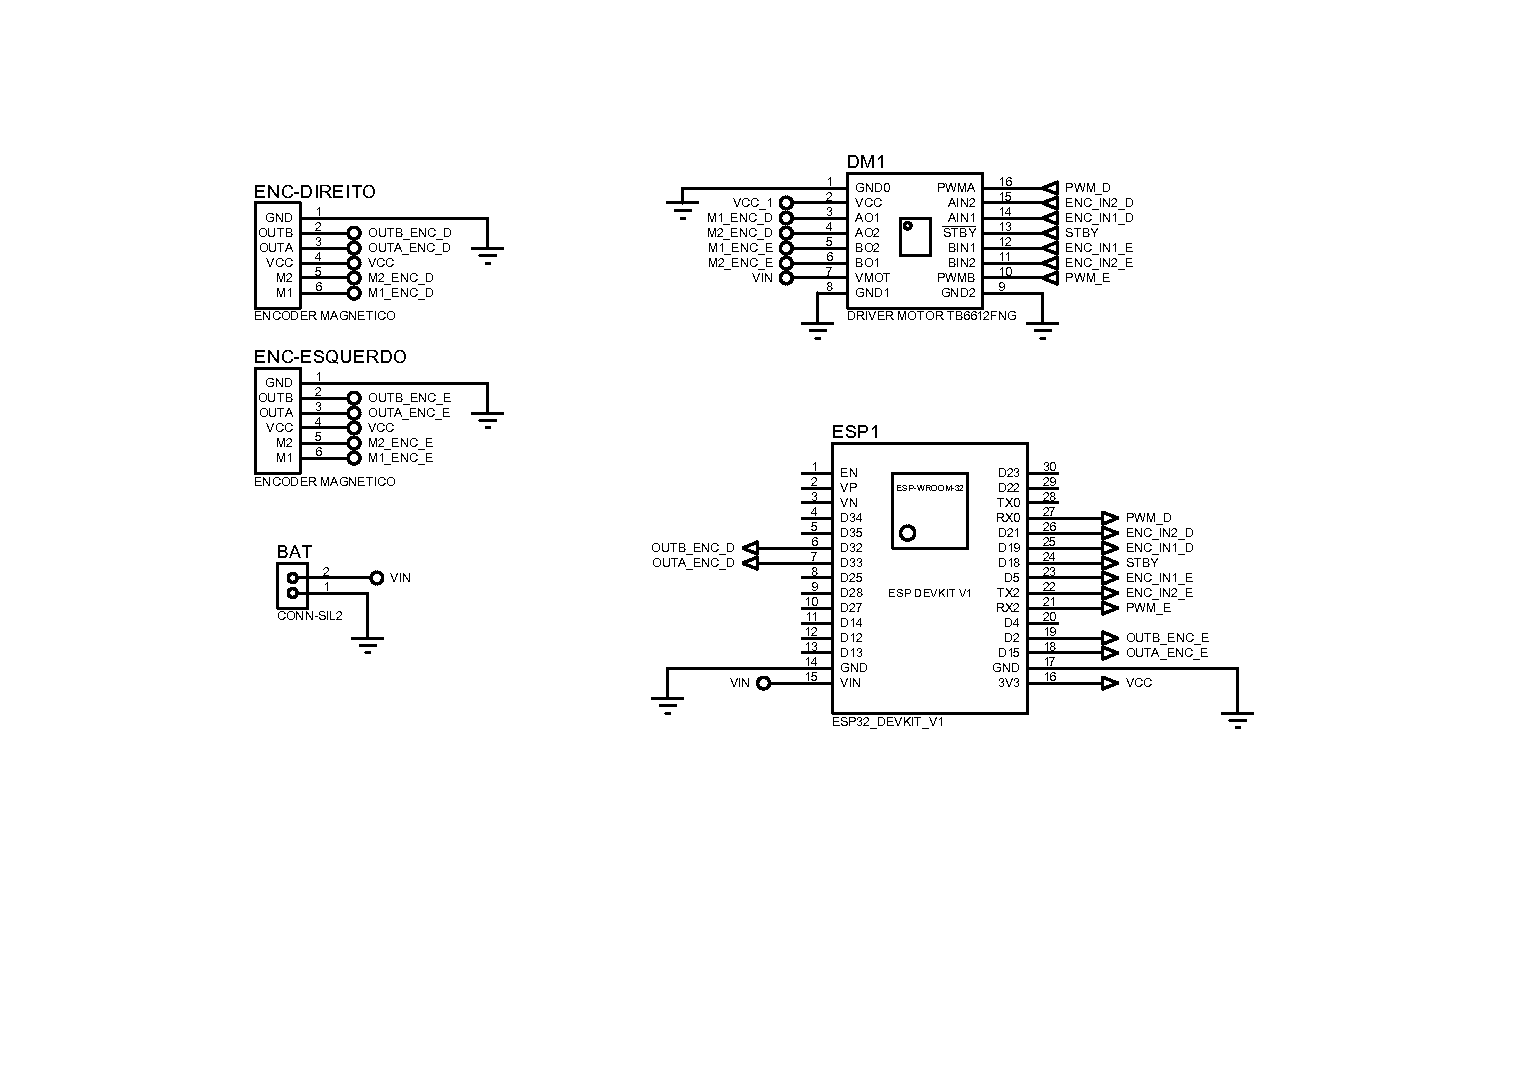
\includegraphics[width=\textwidth]{figuras/eletronica/placa/esquematico_completo.pdf}
            \caption{Esquemático.}
        \end{figure}
        
    \item \textbf{Elaboração do layout}:
        % inserir imagem do layout final aqui
        Este ponto foi o mais crítico nessa tarefa, devido à restrição de tamanho da placa ser de um quadrado com até $55$mm de lado. A solução adotada foi fazer em duas camadas, ou seja, duas placas cobreadas, ambas dupla face, dividindo os componentes. Em uma placa foi comportado o \textit{Driver}, bem como os conectores para os motores com os sensores e os conectores das baterias, e na outra apenas o microcontrolador. Para a conexão entre as placas foi utilizado um conector do tipo \textit{Head}, um macho e uma fêmea. Dessa forma, as placas conseguiram respeitar o limite dimensional e comportar todos os componentes necessários.
    \item \textbf{Realização de testes}:
        % faltou imagem de testes aqui
        Foram realizados testes antes da concepção da PCI, em \textit{Protoboards} para conferir se o circuito está funcionando como esperado e após a confecção, para se verificar a qualidade da confecção das placas.
        
        Também foram realizados testes individuais nos componentes, principalmente nos sensores, com o uso de osciloscópios. Verificou-se o funcionamento correto dos \textit{Encoders} e também conferiu-se se a distância entre os sensores poderia estar gerando interferência um no outro. Os resultados desses testes foram que todos os \textit{encoders} utilizados estão em bom estado, ou seja, funcionando como esperado e a distância que eles ficarão ao serem acomodados na estrutura não causa interferência um no outro.
    \item \textbf{Verificação e validação}
        Após testes individuais, de cada componente, foram realizados testes com a montagem completa, ou seja, os robôs montados por completo com as PCIs, baterias, motores e sensores. A validação foi por meio de controle manual dos robôs e testes simples de leitura de \textit{Encoder}, pois nessa etapa o \textit{Firmware} ainda não havida sido implementado.
\end{enumerate}

\section{O \emph{Firmware}}
% Falar sobre como foi feito a divisão das atividades no microcontrolador
% Mostrar ilustração dessa divisão, para ter-se uma visão global das rotinas e suas relações de dependência

\subsection{Rotina de Calibração}

Rotina responsável por realizar a identificação dos parâmetros do modelo dos motores direito e esquerdo do robô: constante de tempo; ganho de malha aberta; parâmetros do controlador \emph{FeedForward}; velocidade máxima de cada motor. Bem como calcular os ganhos para o controlador \emph{PID} de forma a se obter uma resposta pré-definida em malha fechada.\\

A rotina de calibração consiste em três etapas que são repetidas para todas as configurações: motor direito para frente; motor direito para trás; motor esquerdo para frente e motor esquerdo para trás. Cada etapa é descrita a seguir: \\

% TO DO:
% ORGANIZAR E REPENSAR A FORMA DE EXIBIR AS ETAPAS
% FIGURAS ILUSTRANDO O COMPORTAMENTO GERAL DAS FUNÇÕES QUE ESTÃO SENDO USADAS NA INTERPOLAÇÃO
% PSEUDO CÓDIGOS TALVEZ

\textbf{ETAPA 1.} Estimar a zona morta e o ganho da planta em malha aberta. Para isso é realizado a coleta de $N$ pontos ($\omega$,$u$), o primeiro ponto é coletado para $u = \pm1$(valor máximo no sentido de giro atual) e é realizado sucessivos decréscimos neste valor até a parada do motor ($\omega = 0$). \\

% Aplicar sinal de controle atual ($u_i$);\\
% Aguardar um tempo fixo, pré-determinado, para garantir a leitura de $\omega_{ss}$(velocidade de máxima/velocidade de regime)
% Armazenar ($u_i$,$\omega_{ss}$).\\

A aquisição destes pontos ocorre da maior velocidade para a menor, pois a zona morta será mais baixa neste sentido, devido a inercia do motor.\\

Ao se encerrar a coleta destes pontos ($\omega_{ss} = 0$ detectado) é realizado uma regressão linear por \textit{MMQ}, tendo $\omega$ no eixo das ordenadas e $u$ no eixo das abscisas, o coeficiente angular dessa reta relaciona a velocidade angular ($\omega$) com o sinal de controle ($u$), já o coeficiente linear representa a zona morta, ou seja, o menor $u$ que pode iniciar o giro do motor.

\begin{equation*}
    u(\omega) = a\omega + b
\end{equation*}

Com esses parâmetros dessa reta é possível estimar o ganho de malha aberta da planta da seguinte forma:

\begin{equation*}
    K = \frac{(u_{max} - b)}{a}
\end{equation*}
    
\begin{figure}[H]
    \centering
    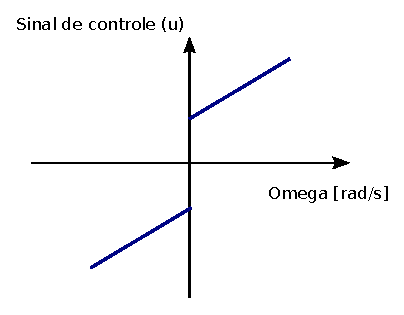
\includegraphics[width=0.5\textwidth]{figuras/ilustracoes/omega_x_sinal_controle.eps}
    \caption{Comportamento da curva $u(\omega)$.}
    \label{fig:ilustracao_omega_x_pwm}
\end{figure}    
    
\textbf{ETAPA 2.} Estimar a constante de tempo. Para obter a constante de tempo da planta na configuração atual, faz-se uso mais uma vez de interpolação por \textit{MMQ} e tira-se proveito do conhecimento do ganho da planta para simplificar e tornar possível essa interpolação de forma simples. Para estimar a constante de tempo obtém-se $M$ pontos ($t$,$\omega$) e aplica-se o \textit{MMQ} para uma interpolação linear, para isso é necessário fazer a seguinte alteração:
    

\begin{align*}
    \omega(t) &= K\left( 1 - e^{-t/T_m} \right)\\
    \ln{\omega(t)} &= \ln\left[K( 1 - e^{-t/T_m})\right]\\
    \ln\left(1 - \frac{\omega(t)}{K} \right) &= -\frac{t}{T_m}\\
    y_{aux}(t) &= -\frac{t}{T_m}
\end{align*}

Convertendo $\omega(t)$ para $y_{aux}(t)$ o coeficiente angular resultante da interpolação linear será: $coef.angular = -\frac{1}{T_m}$, dessa forma obtemos a constante de tempo.\\

\textbf{ETAPA 3.} Calcular os parâmetros do controlador \textit{Feedback}. Como apresentado na seção de referencial teórico é possível relacionar o ganho do controlador proporcional com o polo desejado para o sistema em malha fechada, por meio da relação (??). Esse cálculo só é possível devido a identificação dos parâmetros da planta resultante das etapas anteriores. O polo desejado para todas as configurações da planta é uma constante pré-definida pelo usuário.\\
    

Ao se passar por todas as configurações de motor/sentido a rotina seleciona a menor velocidade máxima apresentada por alguma dessas configurações e armazena esta velocidade como sendo a velocidade máxima atingida pelos motores deste robô, isso é importante, para assegurar que a referencia $\omega_{ref}$ seja factível para todas as configurações. \\

Por fim os resultados são armazenados na memória permanente do microcontrolador, sendo atualizado/sobrescrita apenas ao final da próxima chamada da rotina de calibração.

\subsection{Rotina de Comunicação}
% TODO:
% IDEIA: ILUSTRAR A INTERAÇÃO ENTRE A ROTINA PRINCIPAL E A INTERRUPÇÃO
A rotina de comunicação opera em um \emph{loop} infinito no núcleo principal do microcontrolador e é responsável por tratar os telecomandos recebidos pelo \textit{Bluetooth}. Ao ser identificado um recebimento de mensagem pela sinal de interrupção da comunicação \textit{Bluetooth} é acionado a função de tratamento de interrupção correspondente que possui como única função encaminhar as mensagens válida (verificar cabeçalho) para a rotina principal de comunicação. Isso é feito para evitar sobrecarregar a interrupção, já que ela deve operar em altas frequências.\\

Na rotina principal a mensagem é interpretada e caso ela seja identificado um telecomando válido, será executado a devida resposta, conforme apresentado a seguir.

O protocolo implementado, foi pensado para conter até três grandes campos, o \textbf{\textit{Head}} com 4 bits de preambulo, para ajudar a sincronizar os pacotes, o \textbf{\textit{Cmd}} também com 4 bits, possibilitando assim até 16 comandos distintos e o campos de argumentos com tamanho variável. Foram implementados 7 comandos. 

% Please add the following required packages to your document preamble:
% \usepackage[table,xcdraw]{xcolor}
% If you use beamer only pass "xcolor=table" option, i.e. \documentclass[xcolor=table]{beamer}
\begin{table}[H]
\centering
\begin{tabular}{c|r}
\hline
\rowcolor[HTML]{C0C0C0} 
\multicolumn{1}{|c|}{\cellcolor[HTML]{C0C0C0}DEFINIÇÕES} & \multicolumn{1}{r|}{\cellcolor[HTML]{C0C0C0}VALOR(HEX)} \\ \hline
HEAD & A0 \\
\rowcolor[HTML]{EFEFEF} 
CMD\_REQ\_CAL & 00 \\
CMD\_REQ\_OMEGA & 03 \\
\rowcolor[HTML]{EFEFEF} 
CMD\_CALIBRATION & 04 \\
CMD\_IDENTIFY & 05 \\
\rowcolor[HTML]{EFEFEF} 
CMD\_SET\_POINT & 0A \\
CMD\_CONTROL\_SIGNAL & 0B \\
\rowcolor[HTML]{EFEFEF} 
CMD\_PING & 0F
\end{tabular}
\caption{Definições utilizadas.}
\label{tab:defines}
\end{table}
    
\textbf{Comandos}
\begin{itemize}
    \item \textbf{CMD\_REQ\_CAL}:\\
        \textit{Host} envia, para solicitar os dados provenientes da calibração do controlador \textit{feedforward}. O escravo (robô) envia 4 \emph{floats}, referente aos coeficientes do controlador.
    \item \textbf{CMD\_REQ\_OMEGA}:\\
        \textit{Host} envia, para solicitar as velocidades atuais de ambos os motores, em $rad/s$. O escravo responde com dois \emph{floats}, referentes aos ômegas em cada motor.
    \item \textbf{CMD\_CALIBRATION}:\\
        \textit{Host} envia, para fazer com que o robô inicie sua rotina de calibração do controlador.
    \item \textbf{CMD\_IDENTIFY}:\\
        \textit{Host} envia, fazendo com que o robô inicia sua rotina de identificação. O \textit{Host} deve enviar o \emph{bitstream} da seguinte forma:\\
        
        % Please add the following required packages to your document preamble:
% \usepackage{graphicx}
% \usepackage[table,xcdraw]{xcolor}
% If you use beamer only pass "xcolor=table" option, i.e. \documentclass[xcolor=table]{beamer}
\begin{table}[H]
\centering
\resizebox{\textwidth}{!}{%
\begin{tabular}{|
>{\columncolor[HTML]{C0C0C0}}l |
>{\columncolor[HTML]{C0C0C0}}l |l|l|l|}
\hline
HEAD & CMD\_IDENTIFY & OPTIONS & SETPOINT & STEPTIME \\ \hline
\end{tabular}%
}
\end{table}
        
        Sendo o campos \textbf{options} de 1 byte, contendo a informação de qual motor será feita a identificação e se deve ser usado o controlador.
        
        Ao concluir a rotina de identificação, o robô responde enviando o vetor de ômegas medidos, durante a rotina, para o \textit{host}, que deve estar aguardando recebê-las. A quantidade de dados será $\frac{timeout}{steptime}*4$ bytes, portando o \textit{host} deve estar aguardando exatamente essa quantidade de bytes.
        
        
    \item \textbf{CMD\_SET\_POINT}:\\
        
        % Please add the following required packages to your document preamble:
% \usepackage{graphicx}
% \usepackage[table,xcdraw]{xcolor}
% If you use beamer only pass "xcolor=table" option, i.e. \documentclass[xcolor=table]{beamer}
\begin{table}[H]
\centering
\resizebox{\textwidth}{!}{%
\begin{tabular}{|
>{\columncolor[HTML]{C0C0C0}}c |
>{\columncolor[HTML]{C0C0C0}}c |c|c|c|c|l|l|l|}
\hline
HEAD & CMD\_SET\_POINT & SENSE\_L & OMEGA\_L & SENSE\_R & \multicolumn{4}{c|}{OMEGA\_R} \\ \hline
\end{tabular}%
}

\end{table}
        
        Neste os campos de \textbf{sense\_x} indicam o sentido de rotação do motor, 0 para trás e 1 para rodar para frente (convertidos em sinal dos ômegas de setpoint), portando só ocupam 1 bit, já os campos referentes aos ômegas desejados ocupam 15 bits, sendo assim é possível enviar referências com uma precisão de $1.0/2^{15}$, já que as referências serão enviadas inteiras  (0 - $2^{15}$) e mapeadas de $-1.0$ a $1.0$, indicando uma porcentagem da referência da velocidade máxima do robô. Ou seja os campos referentes aos \textit{setpoints} contêm a porcentagem da velocidade máxima do robô.
        
    \item \textbf{CMD\_CONTROL\_SIGNAL}:\\
        
        O comando difere apenas o campo de \textbf{cmd} do comando anterior. O restante da estrutura é exatamente igual, pois a principal diferença ocorre no microcontrolador. Em vez dos campos referentes aos ômegas serem porcentagens da velocidade máxima que será convertido em \textit{Setpoint} para o controlador, neste comando o robô irá interpretar esses campos como sendo sinais de controle (após convertê-los para \emph{float} de $-1.0$ a $1.0$).
        
    \item \textbf{CMD\_PING}:\\
        Neste comando o \textit{host} pode enviar qualquer mensagem no campo de argumentos, pois o robô irá apenas responder com a mesma mensagem. Este comando é útil para testar conexão e testar a latência da conexão.
    
\end{itemize}

% TABELA TEMPORÁRIA
\begin{table}[H]
\resizebox{\textwidth}{!}{
\begin{tabular}{|l|c|c|l|}
\hline
\multicolumn{1}{|c|}{Command Tag} & \multicolumn{1}{l|}{Hex} & Arg. & \multicolumn{1}{c|}{Description} \\ \hline
CMD\_REQ\_CAL & 0x00 & - & \begin{tabular}[c]{@{}l@{}}Solicita ao microcontrolador que envie os\\ dados da última calibração, que estão armazenados na memória flash.\end{tabular} \\ \hline
 &  &  &  \\ \hline
 &  &  &  \\ \hline
CMD\_REQ\_OMEGA & 0x03 & - & \begin{tabular}[c]{@{}l@{}}Solicita ao microcontrolador que envie as leituras atuais da velocidade\\ de rotação, em rad/s, dos dois motores. O microcontrolador enviará dois\\ floats, sendo primeiro float refererente ao motor esquerdo e o segundo ao\\ motor direito.\end{tabular} \\ \hline
CMD\_CALIBRATION & 0x04 & - & \begin{tabular}[c]{@{}l@{}}Sinaliza para o microcontrolador que ele deve iniciar a rotina de calibração\\ dos parâmetros do controlador, bem como os parâmetros para o filtro de Kalman.\end{tabular} \\ \hline
CMD\_IDENTIFY & 0x05 & - & \begin{tabular}[c]{@{}l@{}}Sinaliza para o microcontrolador que ele deve iniciar a rotina \\ de coleta dos dados  de identificação e ao final deve enviar \\ esses dados para o host.\end{tabular} \\ \hline
 &  &  &  \\ \hline
 &  &  &  \\ \hline
 &  &  &  \\ \hline
 &  &  &  \\ \hline
CMD\_REF & 0x0A & \begin{tabular}[c]{@{}c@{}}ref. Left (15bits)\\ ref.Right (15 bits)\end{tabular} & \begin{tabular}[c]{@{}l@{}}Informa ao microcontrolador qual referência aplicar para \\ o controlador de velocidade de rotação. \\ As referências estão no intervalo {[}-1.0, 1.0{]}.\end{tabular} \\ \hline
CMD\_CONTROL\_SIGNAL & 0x0B & \begin{tabular}[c]{@{}c@{}}pwm. Left (15bits)\\ pwm.Right (15 bits)\end{tabular} & \begin{tabular}[c]{@{}l@{}}Informa ao microcontrolador qual sinal de controle aplicar. \\ Valores no intervalo {[}-1.0, 1.0{]}.\end{tabular} \\ \hline
 &  &  &  \\ \hline
 &  &  &  \\ \hline
CMD\_RESET & 0x0E &  &  \\ \hline
CMD\_PING & 0x0F & mensagem qualquer & Sinaliza para o microcontrolador que ele deve apenas devolver a mensagem para o host. \\ \hline
\end{tabular}
}
\caption{}
\label{tab:command_table}
\end{table}

\subsection{Rotina de Controle}
% TODO:
O controle é executado sozinho no núcleo secundário do ESP32 em \emph{loop} infinito com uma taxa de atualização de $5ms$. A rotina consiste em receber as velocidades providas pela de leitura dos sensores por meio de mensagens entre processos, em seguida é realizado a etapa de controle propriamente dita, que consiste em aplicar a ação do controle \textit{FeedForward} somado a ação do controle de malha fechada, tendo como entrada a última referência de percentual de velocidade lida pela rotina de comunicação multiplicada pela velocidade máxima considerada para a rotação do eixo do motor, para passar a referência para $rad/s$. \\

Ao final do fluxo de controle tem-se o sinal de controle, este por sua vez é utilizado para configurar o sentido de giro e o sinal \emph{PWM} que deve ser aplicado no \emph{Driver} motor correspondente.

% TODO
\begin{algorithm}
\caption{Rotina de Controle}
\label{alg:rotina_leitura_sensores}
\begin{algorithmic}[1]
  \State $lookup\_table \gets $ \{0, 1, -1, 0, 0, 0, 0, 1, 0, 0, 0, -1, 0, 1, -1, 0\}

  % atualiza o codigo
  \State $code \gets (code << 2) + ((READ\_GPIO(CANAL\_A) << 1) + READ\_GPIO(CANAL\_B))$

  \State $t_1 \gets get\_time()$ \Comment{Obtém o tempo atual em segundos.}
  
  \State $\Delta{t} \gets  t_1 - t_0$
  
  \State $t_0 \gets t_1$ \Comment{Atualiza a referência de tempo anterior $t_0$}
  
  \State $\omega_{medido} \gets \frac{2\pi}{N_{PR}*\Delta{t}}$ * $lookup\_table[code]$
  
  \If{ $queue\_input.empty()$ \textbf{E} nunca recebeu} \Comment{Verifica se tem os dados para usar o filtro.}
    \State $queue\_output \gets \omega_{medido}$  \Comment{Coloca o $\omega_{medido}$ na fila de saída e encerra a rotina.}
    \State return;
  \EndIf
  
  \Comment{Caso tenha novos dados (fila de entrada não vazia) atualizar os dados presentes na rotina. Se não usar os dados anteriores.}
  \State $\omega_{ss}$,$\tau$ $\gets  queue\_input$

%   //predição
  \Comment{Etapa de predição.}
  \State $\check{\omega} \gets \omega_{medido}$ + $( \omega_{ss} - \omega_{medido} ) * (1 - exp(-\Delta{t}/\tau))$
  \State $\check{P} \gets \hat{P} + Q$


%   //atualização
  \Comment{Etapa de atualização.}
  \State $K_{gain} \gets \check{P} / (\check{P} + R)$
  \State $\hat{\omega} \gets \check{\omega}$ + $K_{gain} * (\omega_{medido} - \check{\omega})$
  \State $\hat{P} \gets (1 - K_{gain}) * \check{P}$ 
  
  \State $queue\_output \gets \hat{\omega}$
\end{algorithmic}
\end{algorithm}

% ******************************************************************
\subsection{Rotina de Leitura dos Sensores}
% TODO:
% REALIZAR ANÁLISE DE FREQ. MÁXIMA DE OPERAÇÃO DOS ENCODERS VS BANDA DISPONIVEL NAS INTERRUPÇÕES RESPONSAVEIS PELA LEITURA DOS ENCODERS

Há duas interrupções associadas aos sinais provenientes dos \emph{Encoders} rotativos, uma para cada motor, cujo objetivo é medir a velocidade de rotação do eixo do motor ($\omega_{medido}$) bem como aplicar o filtro de \emph{Kalman} para uma melhor estimativa da mesma ($\hat{\omega}$). As interrupções são provocadas pelas bordas dos pulsos de ambos os canais, fazendo com que a resolução do sensor seja utilizada ao máximo, pois dessa maneira os sensores que possuem uma resolução de três pulsos por revolução (em cada canal, ver Figura \ref{fig:ilustracao_uma_revolucao}) consiga acionar doze ($6$) vezes a interrupção que irá computar o $\omega_{motor}$, passando assim a ser ter uma resolução equivalente à seis pulsos por revolução.\\

Para o cálculo do módulo da velocidade de rotação do eixo do motor faz-se uso da medição pelo período do sinal (conforme a Equação \ref{eq:omega_periodimetro}) com os seguintes parâmetros:

\begin{itemize}
    \item $N_{PR} = 6$. Pois são $6$ interrupções por canal (monitorando ambas as bordas de subida e descida);
    \item $T_{hf} = 1\mu{}s$. O contador de alta precisão do $ESP32$ possui, idealmente, uma resolução de $1\mu{}s$ [?].
\end{itemize}

A escolha do método de leitura por periodímetro ao em vez do frequencímetro se deu devido ser possível a leitura imediata da velocidade, pois basta apenas uma interrupção para se ter uma medição e também devido a boa precisão da leitura para abaixas velocidades, mesmo que isso piore para altas velocidades (como mostrado na Equação \ref{eq:erro_quantizacao_periodimetro}). 

\begin{figure}[H]
    \centering
    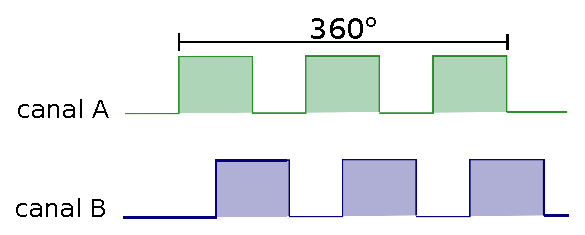
\includegraphics[width=0.5\textwidth]{figuras/ilustracoes/sinal_enquadratura_uma_revolucao.eps}
    \caption{Ilustração do sinal em quadratura em uma revolução completa do eixo do motor no sentido horário.}
    \label{fig:ilustracao_uma_revolucao}
\end{figure}

Já para se obter o sentido de rotação do motor, fez-se uso do padrão \emph{Gray Code} gerado pela diferença de fase entre os diferentes canais de um mesmo sensor. Uma maneira de fazer isso é ler os \emph{GPIO}'s associados aos canais do \emph{Encoder} e verificar o padrão em binário e inferir o sentido de rotação (conforme apresentado anteriormente). Porém esse procedimento apresentou uma alta taxa de erro na inferência do sentido para medias e altas velocidades. \\

A abordagem adotada aqui foi armazenar os dois \emph{bits}(sendo canal A bit mais significado) e concatenar/somar com os últimos dois \emph{bits} (da leitura anterior) deslocados em dois (equivalente à multiplicar por $2^2$ ou operar bit-a-bit: $bits_{anteriores} << 2$), criando assim um padrão com $4$ \emph{bits}, sendo os dois mais significados o padrão da leitura anterior e os dois menos significativos a leitura atual. Esse procedimento é ilustrado para uma rotação no sentido horário e no sentido anti-horário respectivamente nas Tabelas \ref{tab:tabela_gray_code_cw} e \ref{tab:tabela_gray_code_ccw}, dessa forma gera-se quatro($4$) padrões/códigos que caracterizam um tipo de rotação. Esse padrão de $4$\emph{bits} é armazenado de forma estática em um vetor(uma tabela de cola/ \emph{lookup table}) nas rotinas de ambos os motores, esse vetor mapeia o código binário em $1$, $-1$ ou zero para as combinações que não caracterizam um sentido de giro, o sinal do valor corresponde ao sentido horário ou anti-horário e depende do motor. Os vetores \emph{lookup table} para ambos os motores são apresentados  nas Tabela \ref{tab:lookup_table_motor_esquerdo} e \ref{tab:lookup_table_motor_direito}.

% Please add the following required packages to your document preamble:
% \usepackage{graphicx}
\begin{table}[H]
\centering
\resizebox{0.5\textwidth}{!}{%
\begin{tabular}{c|c|c|c|c}
\textbf{$A_{ant}$} & \textbf{$B_{ant}$} & \textbf{$A_{atual}$} & \textbf{$B_{atual}$} & \textbf{DEC} \\ \hline
0 & 0 & 1 & 0 & 2 \\
1 & 0 & 1 & 1 & 11 \\
1 & 1 & 0 & 1 & 13 \\
0 & 1 & 0 & 0 & 4
\end{tabular}%
}
\caption{Codificação de 4 \emph{bits} para a rotação no sentido horário.}
\label{tab:tabela_gray_code_cw}
\end{table}
% Please add the following required packages to your document preamble:
% \usepackage{graphicx}
\begin{table}[H]
\centering
\resizebox{0.5\textwidth}{!}{%
\begin{tabular}{c|c|c|c|c}
\textbf{$A_{ant}$} & \textbf{$B_{ant}$} & \textbf{$A_{atual}$} & \textbf{$B_{atual}$} & \textbf{DEC} \\ \hline
0 & 0 & 0 & 1 & 1  \\
0 & 1 & 1 & 1 & 7  \\
1 & 1 & 1 & 0 & 14 \\
1 & 0 & 0 & 0 & 8 
\end{tabular}%
}
\caption{Codificação de 4 \emph{bits} para a rotação no sentido anti-horário.}
\label{tab:tabela_gray_code_ccw}
\end{table}
% Please add the following required packages to your document preamble:
% \usepackage{graphicx}
\begin{table}[H]
\centering
\resizebox{0.8\textwidth}{!}{%
\begin{tabular}{c|ccccllllllllllll}
\textbf{Índice} & 0 & 1  & 2 & 3 & 4 & 5 & 6 & 7  & 8  & 9 & 10 & 11 & 12 & 13 & 14 & 15 \\ \hline
\textbf{Valor}  & 0 & -1 & 1 & 0 & 1 & 0 & 0 & -1 & -1 & 0 & 0  & 1  & 0  & 1  & -1 & 0 
\end{tabular}%
}
\caption{\emph{Lookup table} para o motor esquerdo.}
\label{tab:lookup_table_motor_esquerdo}
\end{table}
% Please add the following required packages to your document preamble:
% \usepackage{graphicx}
\begin{table}[H]
\centering
\resizebox{0.8\textwidth}{!}{%
\begin{tabular}{c|ccccllllllllllll}
\textbf{Índice} & 0 & 1  & 2 & 3 & 4 & 5 & 6 & 7  & 8  & 9 & 10 & 11 & 12 & 13 & 14 & 15 \\ \hline
\textbf{Valor}  & 0 & 1 & -1 & 0 & -1 & 0 & 0 & 1 & 1 & 0 & 0  & -1  & 0  & -1  & 1 & 0 
\end{tabular}%
}
\caption{\emph{Lookup table} para o motor direito.}
\label{tab:lookup_table_motor_direito}
\end{table}

Com a \emph{lookup table} e o módulo da velocidade é possível calcular a velocidade de rotação da seguinte forma:

\begin{equation}
    \omega_{medido} = \frac{2\pi}{N_{PR}\Delta{t}}table[code]
\end{equation}

Sendo,

\begin{equation*}
    \Delta{t} = nT_{hf}
\end{equation*}

Uma vez calculado o $\omega_{medido}$, calcula-se em seguida a melhor estimativa para $\omega$ ($\hat{\omega}$) utilizando-se o filtro de \emph{Kalman}. Para isso é considerado que o sistema $\omega(t)$ possui um comportamento de primeira ordem (conforme Equação \ref{eq:motor_transf_func}), fazendo com que as variáveis do filtro sejam:

\begin{equation*}
\begin{cases}
    \textbf{x}_k = \left[ \omega_k \right]\\
    z_k = x_k = \omega_k\\
    F_k = 1\\
    H_k = 1
\end{cases}
\end{equation*}

Modelo da \textbf{medição}:
\begin{align*}
z_k = \omega_{medido}
\end{align*}

Com isso a etapa de \textbf{predição} do filtro torna-se:
% MUDAR O SIMBOLO QUE FAZ REFERENCIA À ENTRADA (u) DE ENTRADA
\begin{align*}
    \check{\omega}_{k|k-1} &= \hat{\omega}_{k-1} + u_k\left( 1 - e^{-\Delta{t}/T_m} \right)\\
    \check{P}_{k|k-1} &= \hat{P}_{k-1} + Q_k
\end{align*}

Sendo $u_k$ a entrada no instante $k$.\\

E a etapa de atualização \textbf{Atualização} é:

\begin{align*}
K_k &= \check{P}_k \left( \check{P}_k + R_k \right)^{-1} = \frac{\check{P}_k}{\check{P}_k + R_k}\\
\hat{\omega}_k &= \check{\omega}_k + K_k \left( \omega_{k_{medido}} - \check{\omega}_k \right)\\
\hat{P}_k &= \left( 1 - K_k \right) \check{P}_k
\end{align*}

Os parâmetros do filtro foram sintonizados experimentalmente.\\

Um pseudo código ilustrando a rotina de leitura dos sensores é apresentado a seguir:

\begin{algorithm}
\caption{Rotina de Leitura dos Sensores}
\label{alg:rotina_leitura_sensores}
\begin{algorithmic}[1]
  \State $lookup\_table \gets $ \{0, 1, -1, 0, 0, 0, 0, 1, 0, 0, 0, -1, 0, 1, -1, 0\}

  % atualiza o codigo
  \State $code \gets (code << 2) + ((READ\_GPIO(CANAL\_A) << 1) + READ\_GPIO(CANAL\_B))$

  \State $t_1 \gets get\_time()$ \Comment{Obtém o tempo atual em segundos.}
  
  \State $\Delta{t} \gets  t_1 - t_0$
  
  \State $t_0 \gets t_1$ \Comment{Atualiza a referência de tempo anterior $t_0$}
  
  \State $\omega_{medido} \gets \frac{2\pi}{N_{PR}*\Delta{t}}$ * $lookup\_table[code]$
  
  \If{ $queue\_input.empty()$ \textbf{E} nunca recebeu} \Comment{Verifica se tem os dados para usar o filtro.}
    \State $queue\_output \gets \omega_{medido}$  \Comment{Coloca o $\omega_{medido}$ na fila de saída e encerra a rotina.}
    \State return;
  \EndIf
  
  \Comment{Caso tenha novos dados (fila de entrada não vazia) atualizar os dados presentes na rotina. Se não usar os dados anteriores.}
  \State $\omega_{ss}$,$\tau$ $\gets  queue\_input$

%   //predição
  \Comment{Etapa de predição.}
  \State $\check{\omega} \gets \omega_{medido}$ + $( \omega_{ss} - \omega_{medido} ) * (1 - exp(-\Delta{t}/\tau))$
  \State $\check{P} \gets \hat{P} + Q$


%   //atualização
  \Comment{Etapa de atualização.}
  \State $K_{gain} \gets \check{P} / (\check{P} + R)$
  \State $\hat{\omega} \gets \check{\omega}$ + $K_{gain} * (\omega_{medido} - \check{\omega})$
  \State $\hat{P} \gets (1 - K_{gain}) * \check{P}$ 
  
  \State $queue\_output \gets \hat{\omega}$
\end{algorithmic}
\end{algorithm}

% \subsubsection{Rotina de Telemetria}
% TODO:
% NOTA:
% Não sei se seria interessante falar dessa. Ao ser ativada ela inicia o armazenamento de vários dados, como velocidades, setpoint, velocidade filtrada, velocidade não filtrada, variáveis do filtro... grava esses dados durante x segundos e ao final envia tudo ao host via bluetooth

% Resultados
\chapter[Resultados]{Resultados}
\label{ch:resultados}

% APENAS PARA ILUSTRAR O TIPO DE PLOTS QUE PRETENDO COLOCAR
% CONSIGO REFAZER QUALQUER PLOT FACILMENTE
% TENHO INFORMAÇÃO/DADOS PARA GERAR DIVERSOS PLOTS E TESTES OFFLINE

% OBJETIVO:
% 1) MOSTRAR O RESULTADO DA CALIBRAÇÃO (CURVA ESTIMADA X DADOS BRUTOS)
% 2) MOSTRAR O RESULTADO DA FILTRAGEM; COMPARAR COM FILTOS SIMPLES (POSSO APLICAR OS FILTROS OFFLINE NOS DADOS COLETADOS)
% 3) MOSTRAR O RESULTADO DO CONTROLE, PRINCIPALMENTE COM O INTUITO DE DIMINUIR AS ASSIMETRIAS DOS MOTORES

% MOSTRAR:
% RESPOSTAS PARA DIFERENTES CONFIGURAÇÕES DE MOTOR-SENTIDO E COM DIFERENTES REFERENCIAS/SINAIS DE CONTROLE PARA:
% CURVA ESTIMADA X SEM FILTRO X COM FILTRO
% 


\section{Resultados da calibração}

\begin{figure}[H]
    \centering
    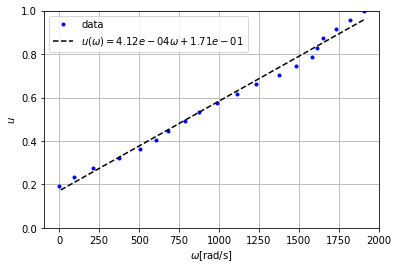
\includegraphics[width=13cm]{figuras/resultados/plot_test_calibration_result_feedforward.png}
    \caption{TESTE: RESULTADO DA IDENTIFICAÇÃO/CALIBRAÇÃO}
\end{figure}

\begin{figure}[H]
    \centering
    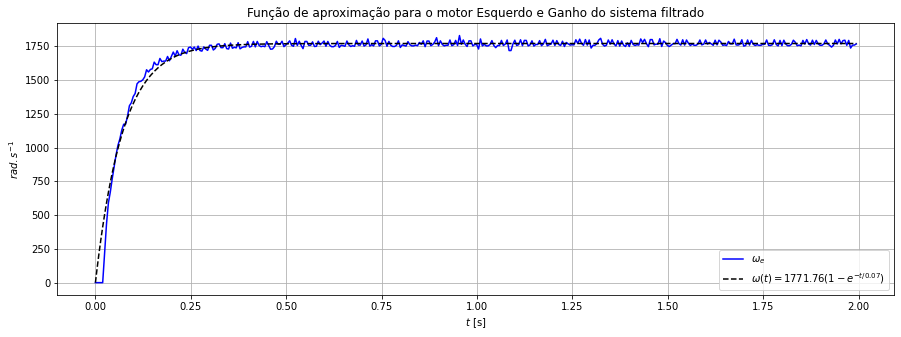
\includegraphics[width=13cm]{figuras/resultados/plot_test_identificacao.png}
    \caption{TESTE: RESULTADO DA IDENTIFICAÇÃO/CALIBRAÇÃO}
\end{figure}

\section{Filtragem da velocidade}
% MOSTRAR A FILTRAGEM COM DIFERENTES PARÂMETROS:
% sintonizando a incerteza da medição e do modelo (Q e R)

\begin{figure}[H]
    \centering
    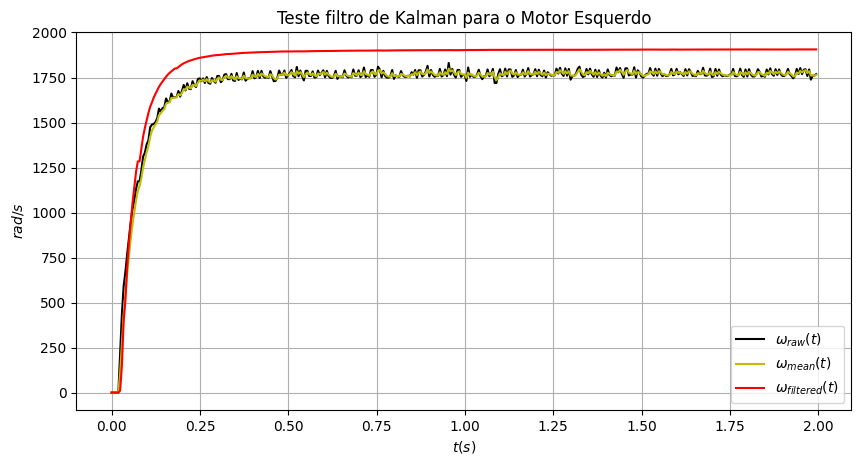
\includegraphics[width=13cm]{figuras/resultados/plot_test_media_x_kalman.png}
    \caption{TESTE: MEDIA VS KALMAN}
\end{figure}

\section{Respostas do sistema com os controladores}


\begin{figure}[H]
    \centering
    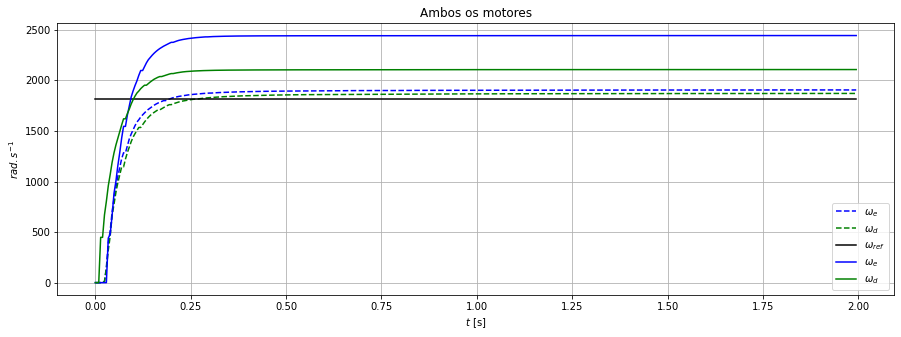
\includegraphics[width=13cm]{figuras/resultados/plot_test.png}
    \caption{TESTE: COM CONTROLE VS SEM CONTROLE}
\end{figure}

\begin{figure}[H]
    \centering
    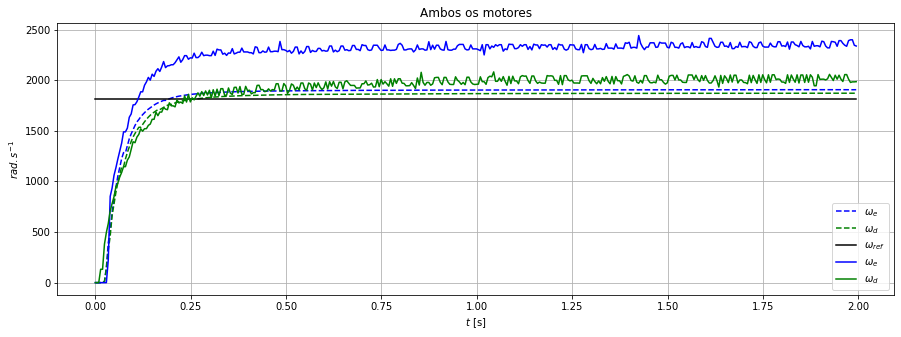
\includegraphics[width=13cm]{figuras/resultados/plot_test_antes_x_depois.png}
    \caption{TESTE: ANTES X DEPOIS}
\end{figure}


% Discussão
\chapter[Discussão]{Discussão}
\label{ch:Discussão}

% Consiste na análise e comparação entre os resultados obtidos pelo autor e os encontrados na literatura, avaliando e criticando a exatidão dos dados obtidos e a concordância ou não com outros autores. A metodologia utilizada e as implicações práticas da pesquisa devem ser discutidas, podendo apresentar propostas que visem contribuir para as soluções dos problemas detectados, ou sugerir outros.

\lipsum[2-3]


% Conclusão
\chapter[Conclusão]{Conclusão}
\label{ch:conclusao}
% TER EM MENTE:
% Deve ser fundamentada nos resultados, contendo deduções lógicas que correspondam aos objetivos do tema proposto e às expectativas descritas pelo autor na introdução do trabalho. É a resposta à pergunta da pesquisa – o objetivo do TCC. A conclusão é a fase final de toda a argumentação; relaciona as diversas partes da argumentação, amarra as ideias desenvolvidas. É a síntese de toda reflexão e, em certo sentido, é um regresso à introdução: fecha-se o começo, o que se propôs na introdução.

% Escreva suas conclusões, limitações do seu trabalho, contribuições, trabalhos futuros, etc.

Pelos exposto no \autoref{ch:resultados} nota-se que: A aproximação do comportamento dos motores para um sistema de primeira ordem, mostrou-se ser suficientemente para todos os experimentos realizados (como esperado, conforme apresentado na \autoref{sec:motor_ref_teo}); O uso do filtro de \emph{Kalman} para estimar a velocidade de rotação dos motores, mostrou-se extremamente eficiente, pois conseguiu reduzir quase que completamente os erros de quantização, mesmo com medições provenientes de sensores de baixa resolução e operando em altas velocidades (pior condição para a leitura de \emph{Encoders} pelo método da medição de períodos); O controlador \emph{Feedforward} em conjunto com o controlador proporcional (\emph{Backward}) também mostrou bons resultados, conseguindo rastrear a referência com uma margem de erro relativamente baixa, além de atingir os tempos de respostas desejados (constante de tempo desejada) e contornar as pertubações externas (como mostrado principalmente no experimento 4 nas Figuras \ref{fig:exp04:antes_vs_depois}).\\

Conclui-se portanto que o sistema proposto é capaz de oferecer boas estimativas de velocidades por meio do filtro de \emph{Kalman}, mesmo para sensores com baixa resolução. E que o sistema de controle (fazendo uso dessas estimativas) é capaz de reduzir as assimetrias do par motor-roda de (mas não limitando-se) robôs com acionamento diferencial. Além disso, o sistema proposto apresentou-se como uma solução simples o suficiente para conseguir ser implementado em um \emph{Hardware} com recursos limitados, como um  microcontrolador.\\

Faz-se necessário também algumas observações importantes a respeito dos experimentos e de suas análises apresentados no capítulo anterior, são elas: A escolha de se trabalhar com as velocidades no eixo do motor antes da caixa de redução fez com que os valores em módulo dessas velocidades fossem altos, dificuldade um pouco a análise visual dos gráficos, fazendo (por exemplo) com que erros absolutos no rastreio da referência seja mascarado devido a escala dos gráficos. Outro ponto, é com relação à variedade dos experimentos, os quatro experimentos mostram pouca diferença entre si. Provavelmente isso é devido ao fato de que a maioria deles foram realizados com os robôs suspensos (sem contato com o chão), apenas o experimento 4 foi feito com um robô em contato com o chão (situação de operação normal do robô). O motivo disso foram problemas técnicos encontrados durante a fase de experimentação e testes, que fez com que dois dos três robôs disponíveis não conseguissem operar normalmente, limitando assim as possibilidades de testes.\\

O presente trabalho possuí como objetivos futuros: A adição da ação integral (controlador PI) no sistema de controle, para eliminar o erro residual que o controlador \emph{Feedforward} não está sendo capaz de eliminar e a calibração automática (dinâmica), principalmente do ganho do sistema, por meio da técnica de mínimos quadrados recursivos, como apresentado em por alguns dos trabalhos descritos na \autoref{sec:trabalhos_relacionados}.




% ----------------------------------------------------------
% ELEMENTOS PÓS-TEXTUAIS

% 
\postextual

% Referências bibliográficas
%\addcontentsline{toc}{chapter}{Referências Bibliográficas}

\bibliographystyle{abntex2-alf}
%\bibliographystyle{unsrt}
\bibliography{bibliografia/referencias}

\end{document}
